\section{Metriche di Valutazione}
In questa sezione vengono analizzate le prestazioni dei modelli attraverso i grafici delle principali metriche di valutazione: ROUGE, WER e cosine similarity. 
Queste metriche sono state scelte per misurare in modo accurato la qualit\`a dei riassunti generati, confrontandoli con quelli di riferimento.\\
Le valutazioni sono state effettuate utilizzando il dataset di test, che non \`e stato utilizzato durante l'addestramento del modello.\\
Durante la fase di inferenza, sono stati generati 1000 riassunti a partire dai dati di test.

\subsection{ROUGE (Recall-Oriented Understudy for Gisting Evaluation)}
Sono state calcolate tre varianti di ROUGE:
\begin{itemize}
    \item ROUGE-1: confronta unigrammi tra il riassunto generato e quello di riferimento
    \item ROUGE-2: considera bigrammi per valutare la similarit\`a tra i due testi
    \item ROUGE-L: confronta la sottosequenza pi\`u lunga comune tra i due testi
\end{itemize}    

I grafici nella Figura \ref{fig:rouge_comparison} confrontano le performance in termini di ROUGE-1, ROUGE-2 e ROUGE-L per i quattro modelli. Il modello Seq2SeqBiLSTM mostra un miglioramento nei punteggi ROUGE rispetto al Seq2SeqLSTM e al Seq2SeqLSTMGlove, indicando una maggiore capacit\`a di catturare similarit\`a lessicali.
\begin{figure}[H]
    \centering
    \begin{subfigure}{0.24\textwidth}
        \centering
        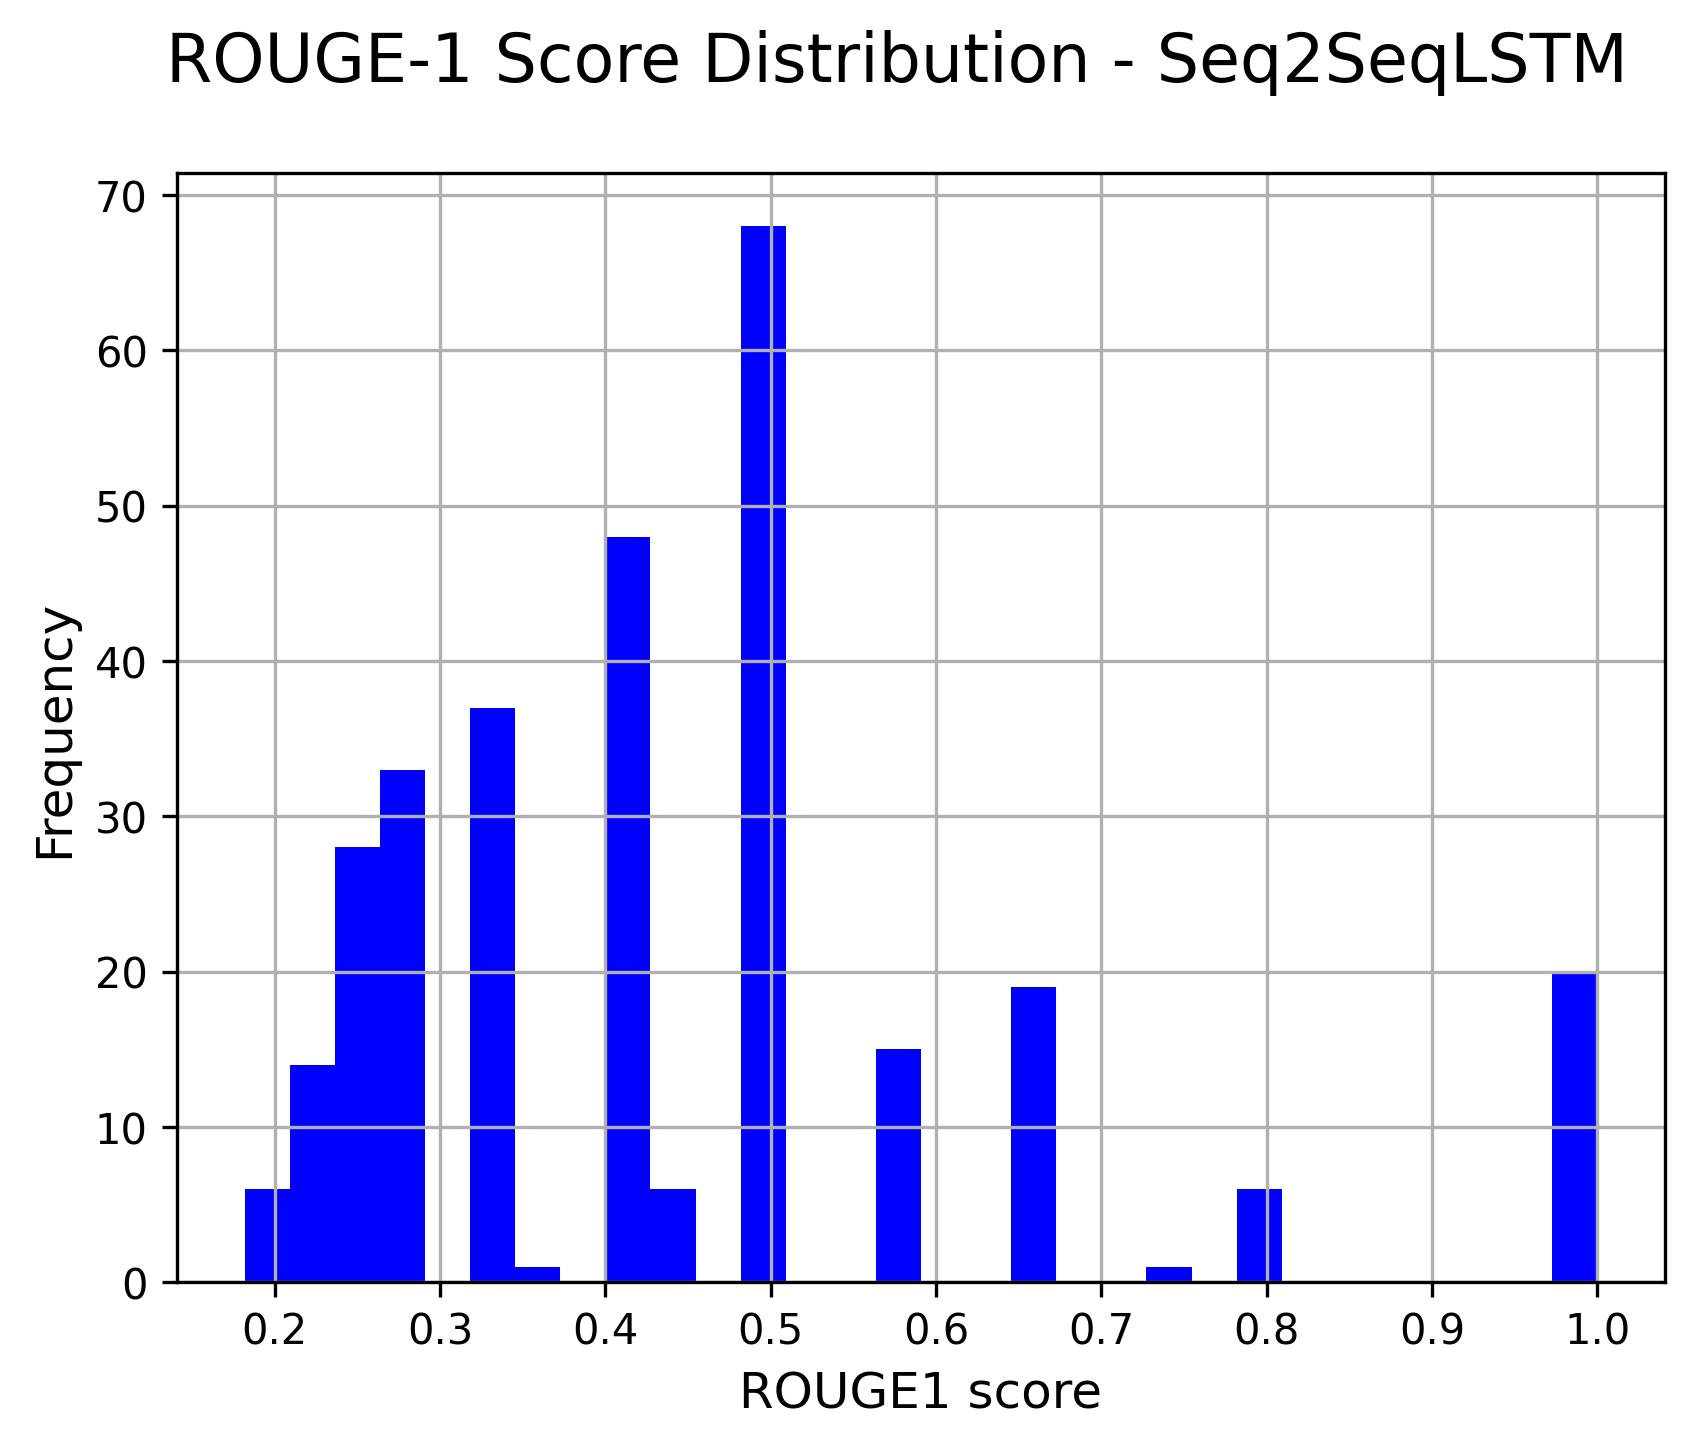
\includegraphics[width=\textwidth]{media/Seq2SeqLSTM_rouge1_scores.png}
        \caption{ROUGE-1 Seq2SeqLSTM}
    \end{subfigure}
    \hfill
    \begin{subfigure}{0.24\textwidth}
        \centering
        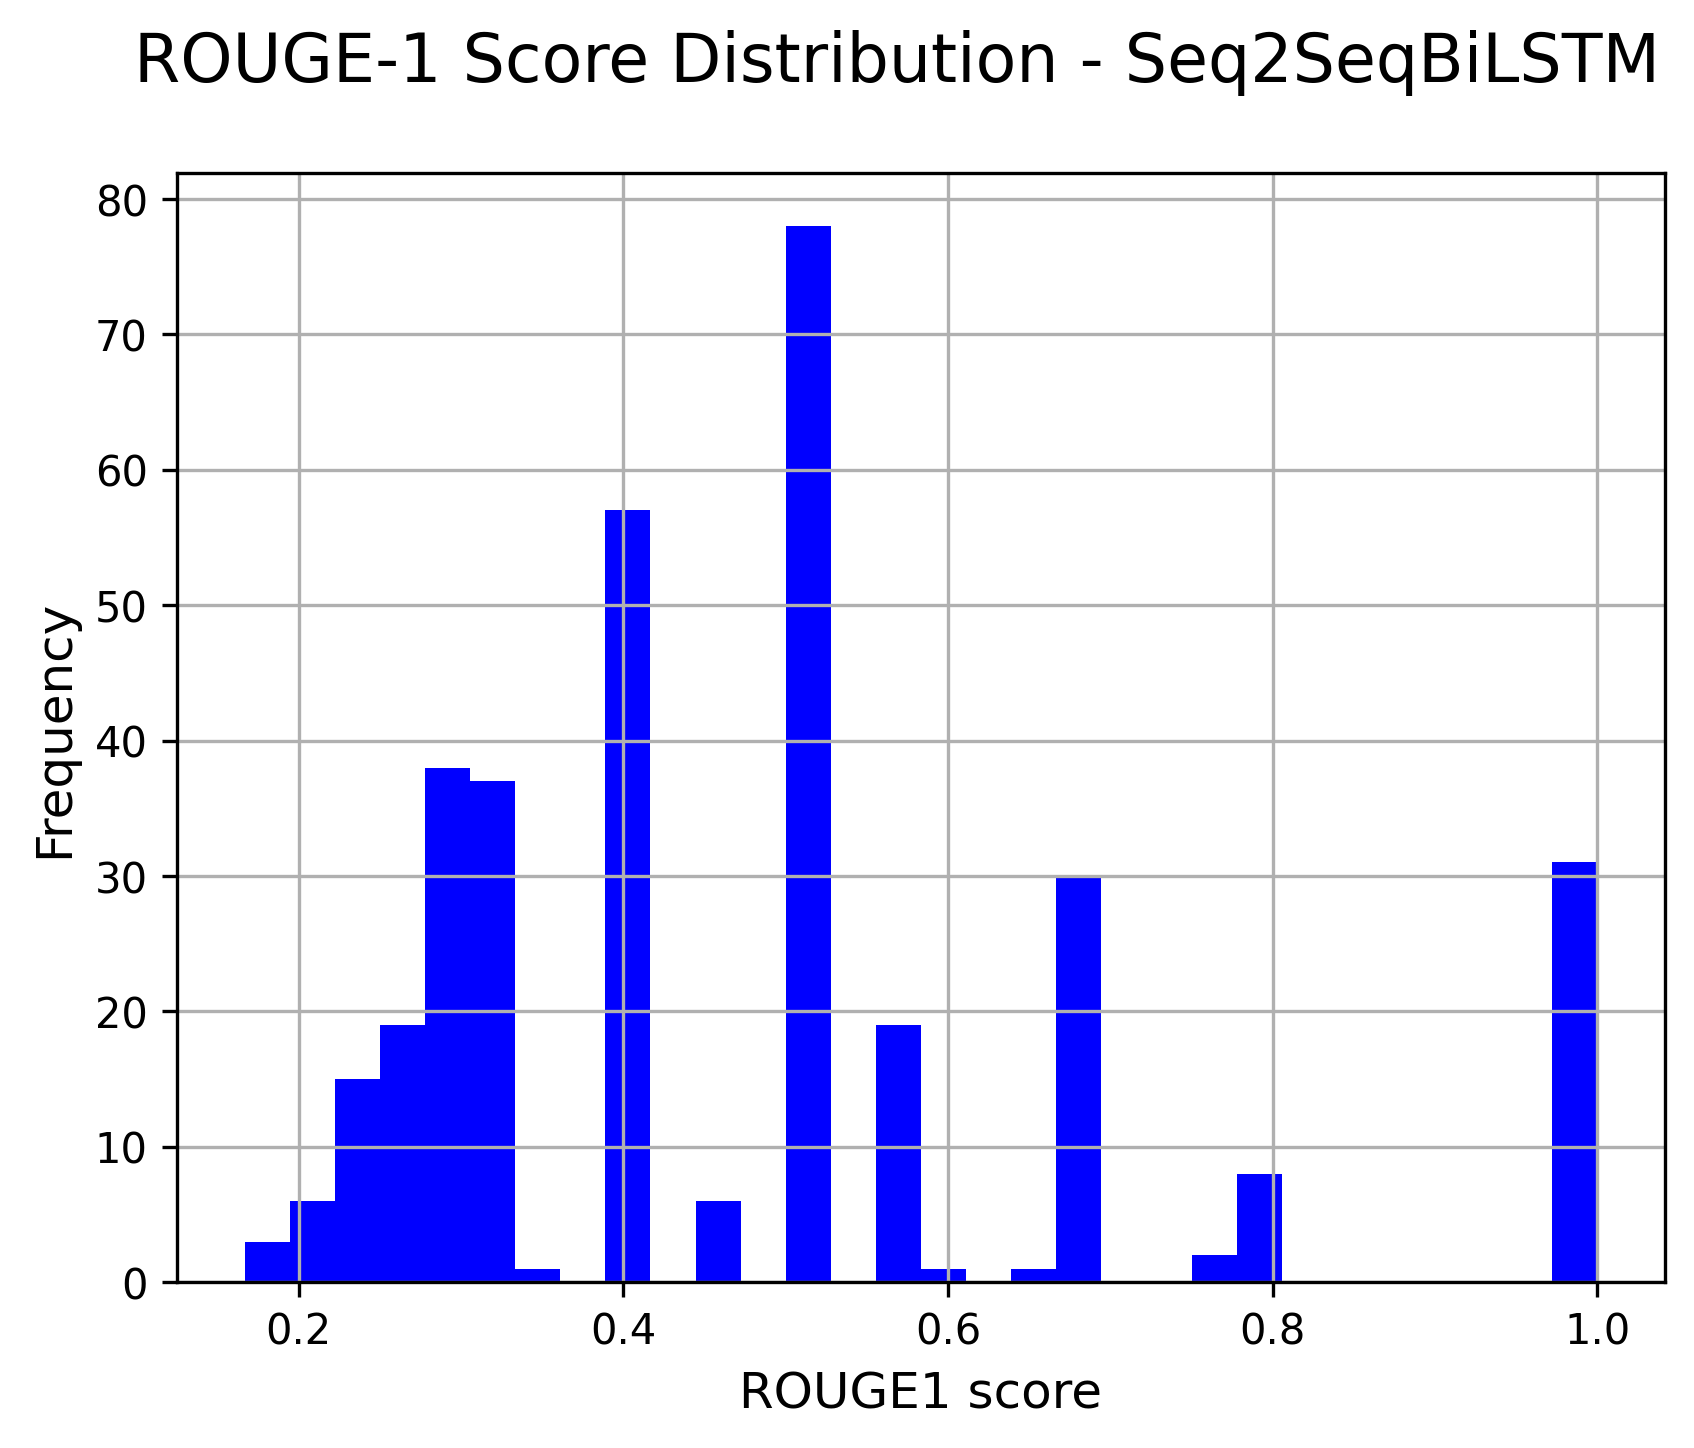
\includegraphics[width=\textwidth]{media/Seq2SeqBiLSTM_rouge1_scores.png}
        \caption{ROUGE-1 Seq2SeqBiLSTM}
    \end{subfigure}
    \hfill
    \begin{subfigure}{0.24\textwidth}
        \centering
        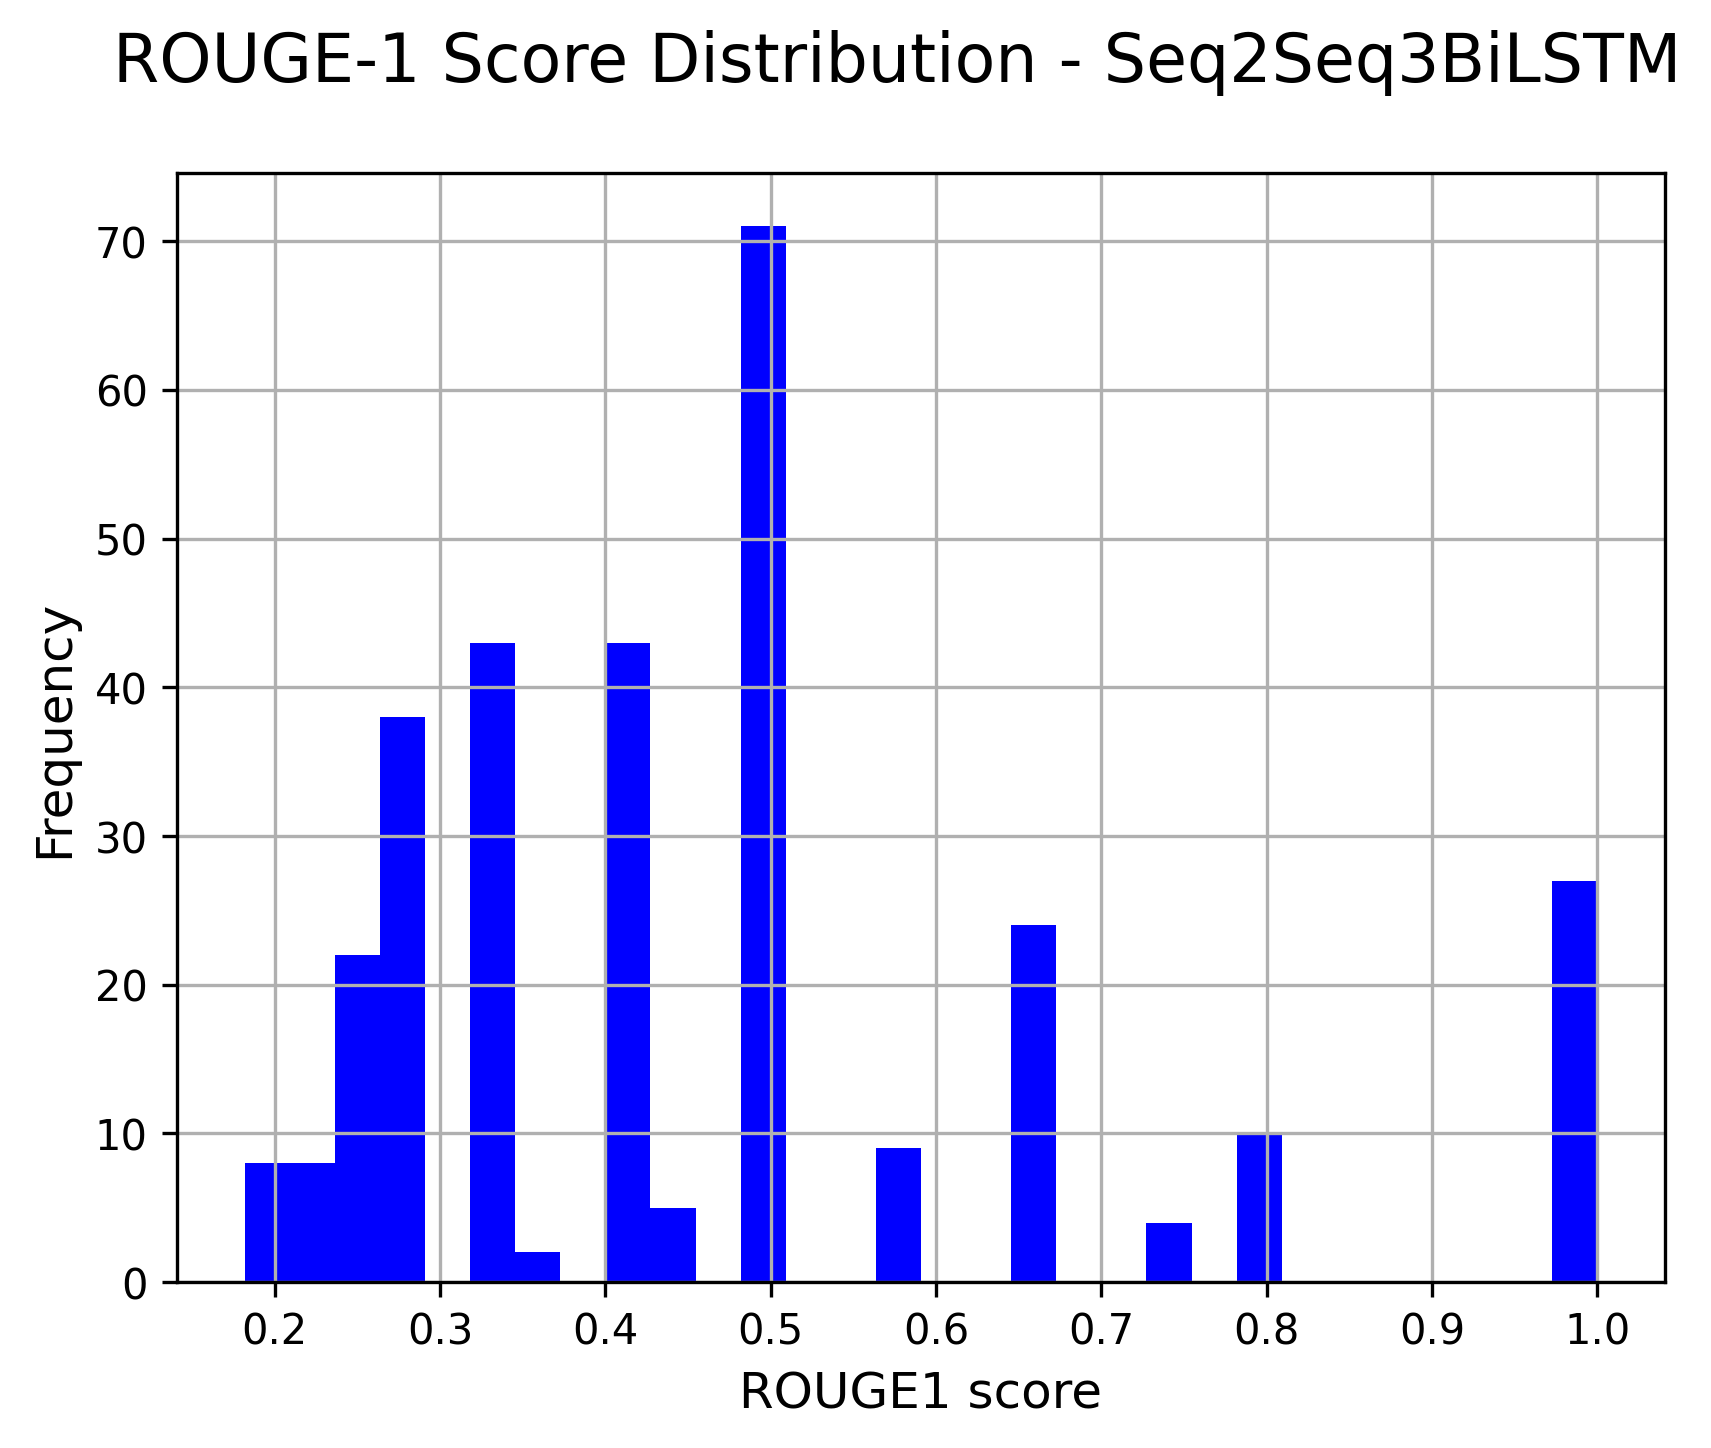
\includegraphics[width=\textwidth]{media/Seq2Seq3BiLSTM_rouge1_scores.png}
        \caption{ROUGE-1 Seq2Seq3BiLSTM}
    \end{subfigure}
    \hfill
    \begin{subfigure}{0.24\textwidth}
        \centering
        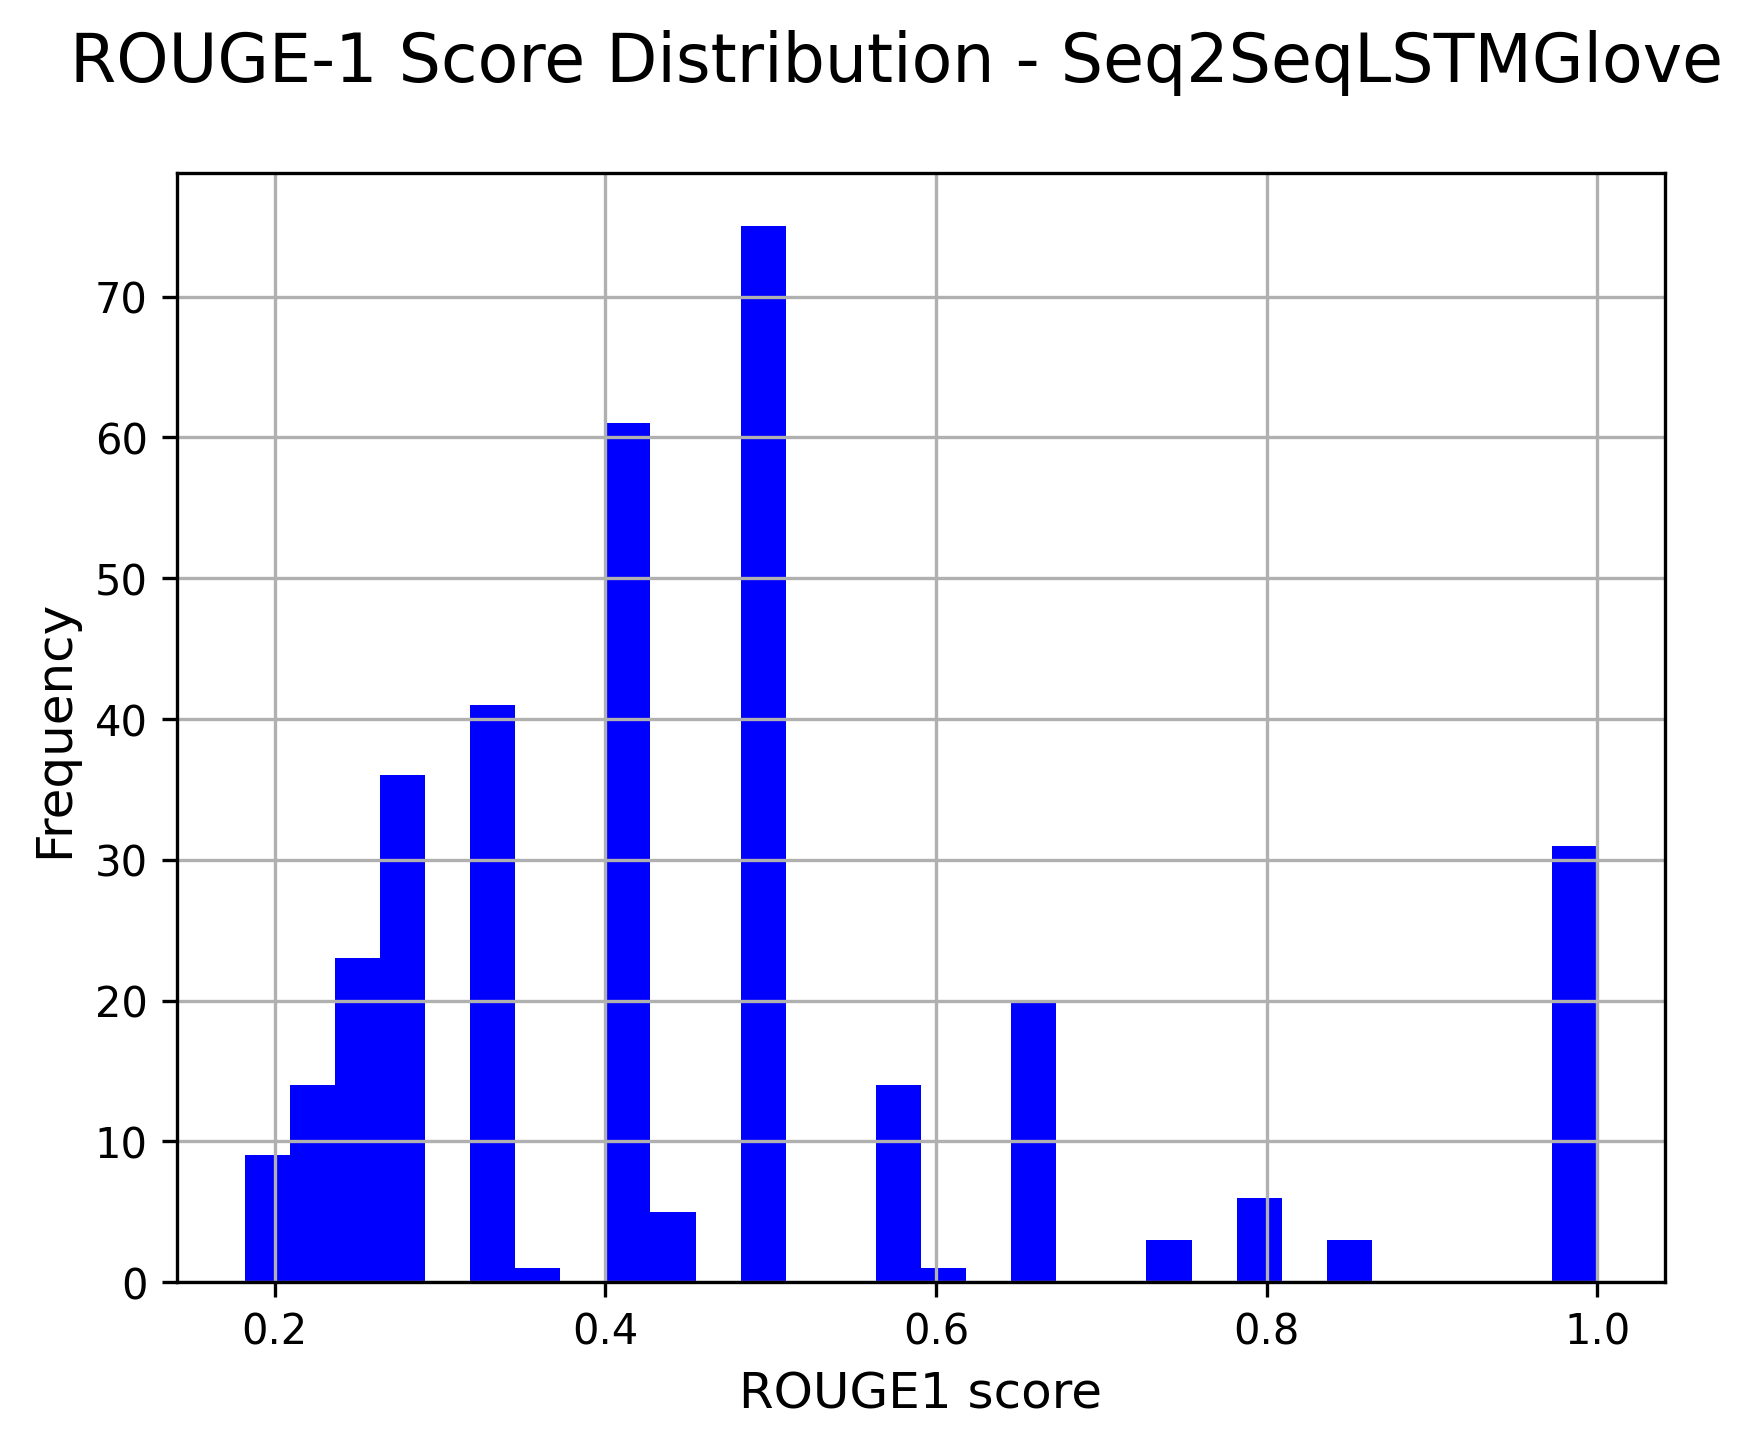
\includegraphics[width=\textwidth]{media/Seq2SeqLSTMGlove_rouge1_scores.png}
        \caption{ROUGE-1 Seq2SeqLSTMGlove}
    \end{subfigure}
    \hfill
    \begin{subfigure}{0.24\textwidth}
        \centering
        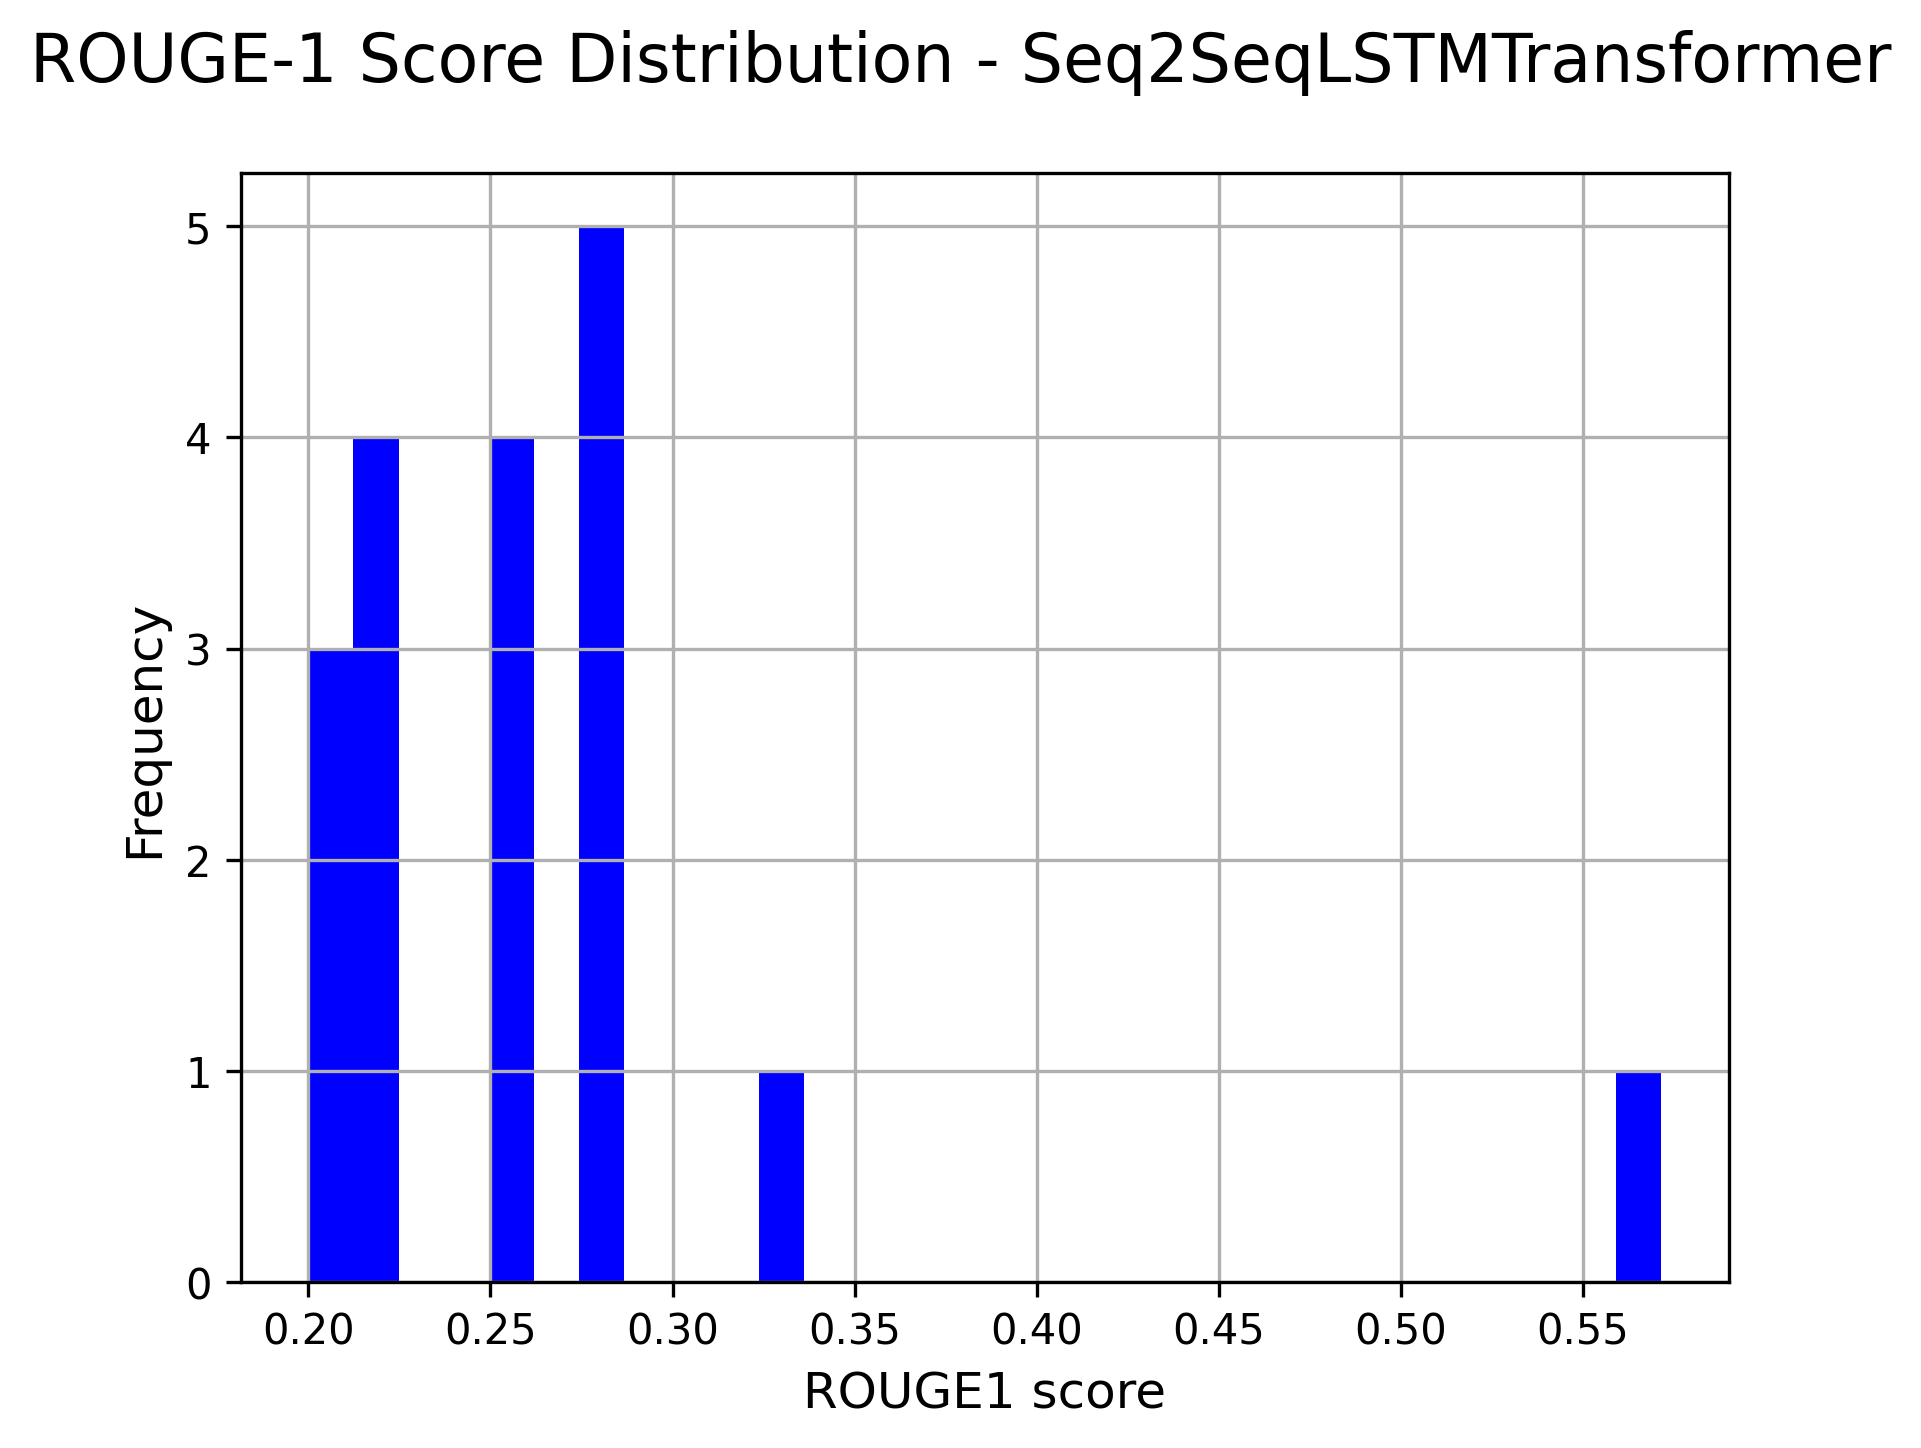
\includegraphics[width=\textwidth]{media/Seq2SeqLSTMTransformer_rouge1_scores.png}
        \caption{ROUGE-1 Seq2SeqLSTMTransformer}
    \end{subfigure}

    \begin{subfigure}{0.24\textwidth}
        \centering
        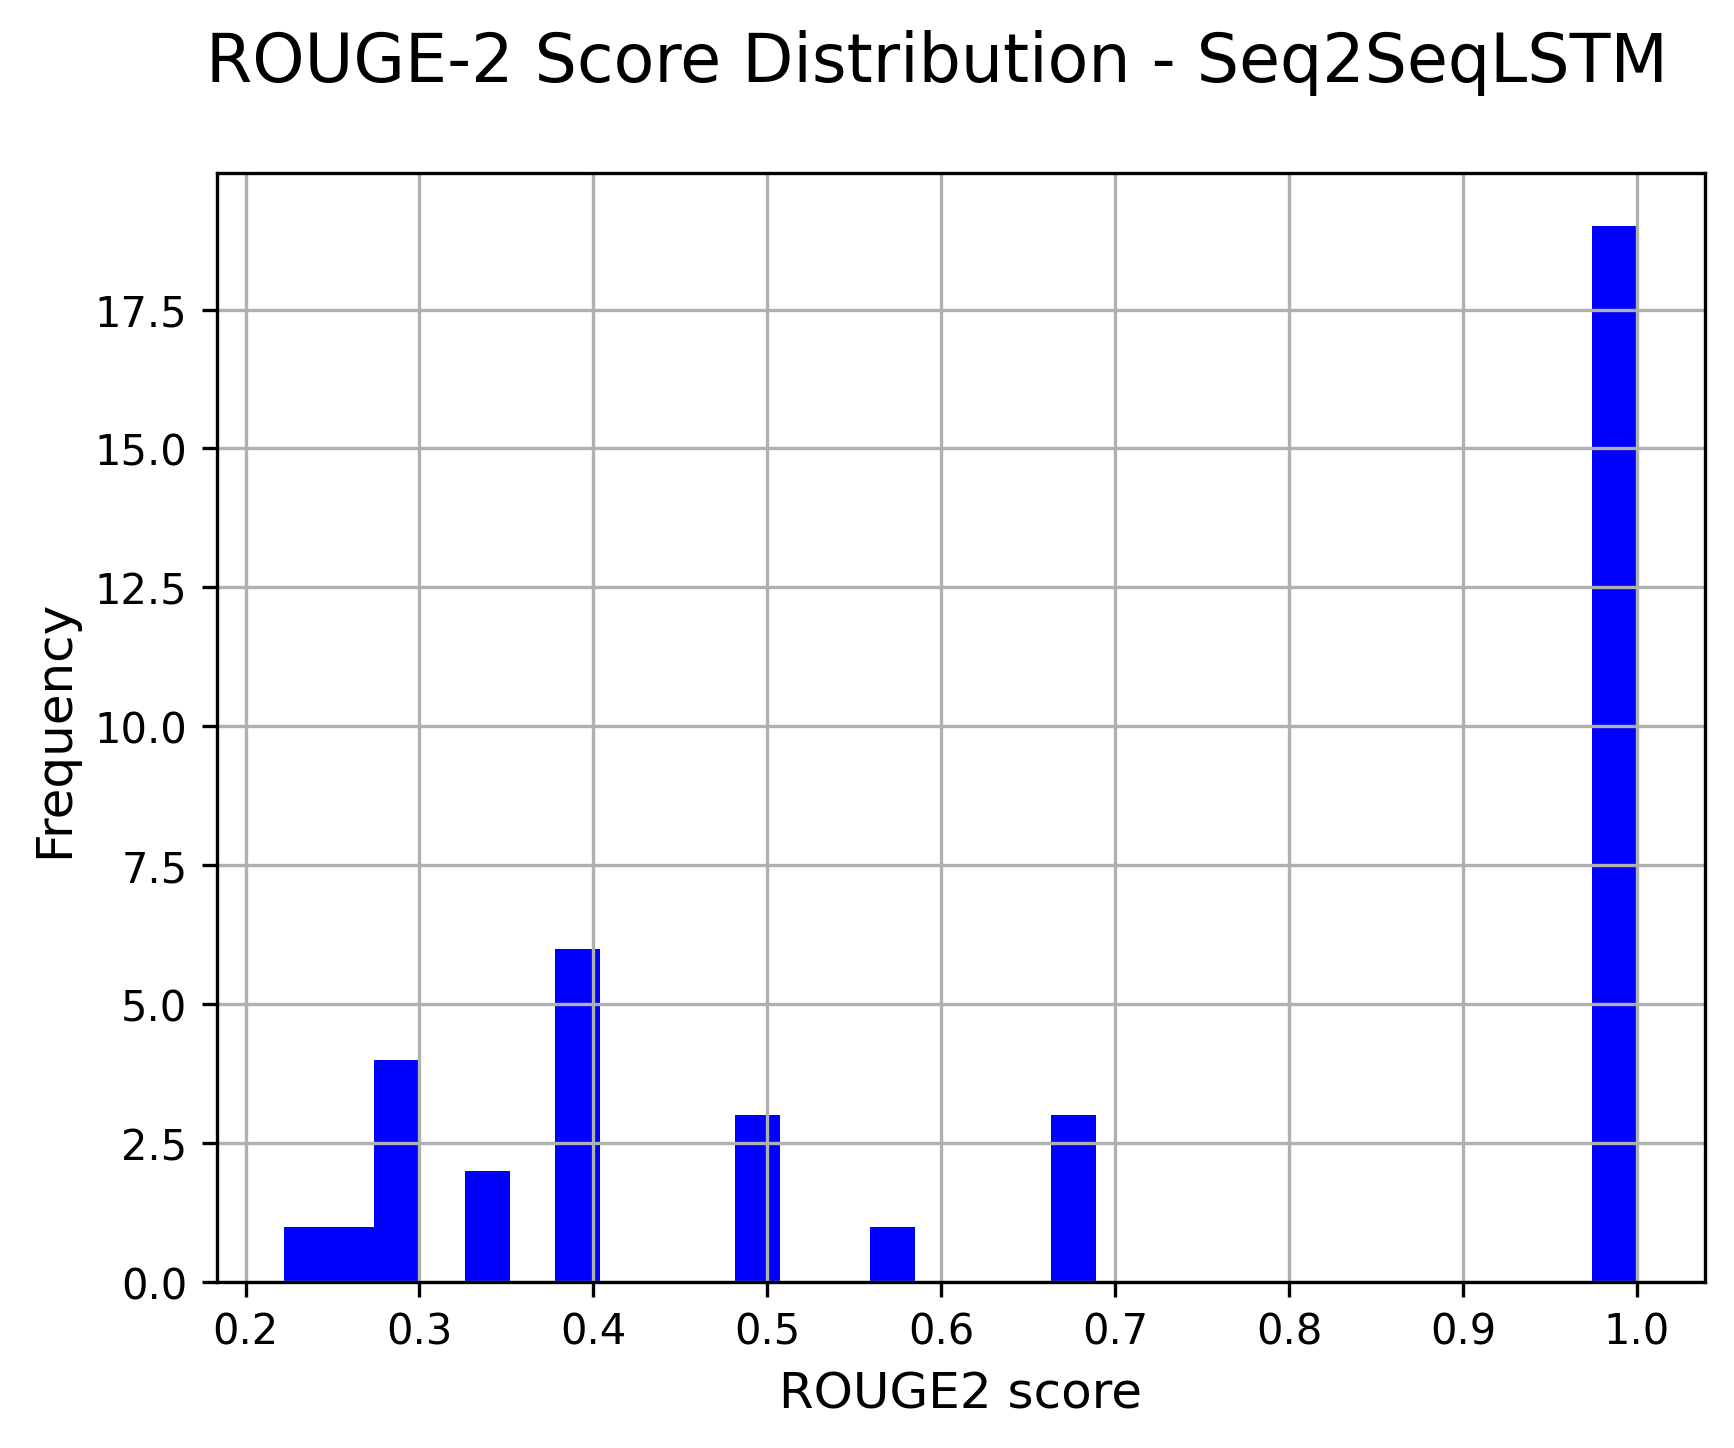
\includegraphics[width=\textwidth]{media/Seq2SeqLSTM_rouge2_scores.png}
        \caption{ROUGE-2 Seq2SeqLSTM}
    \end{subfigure}
    \hfill
    \begin{subfigure}{0.24\textwidth}
        \centering
        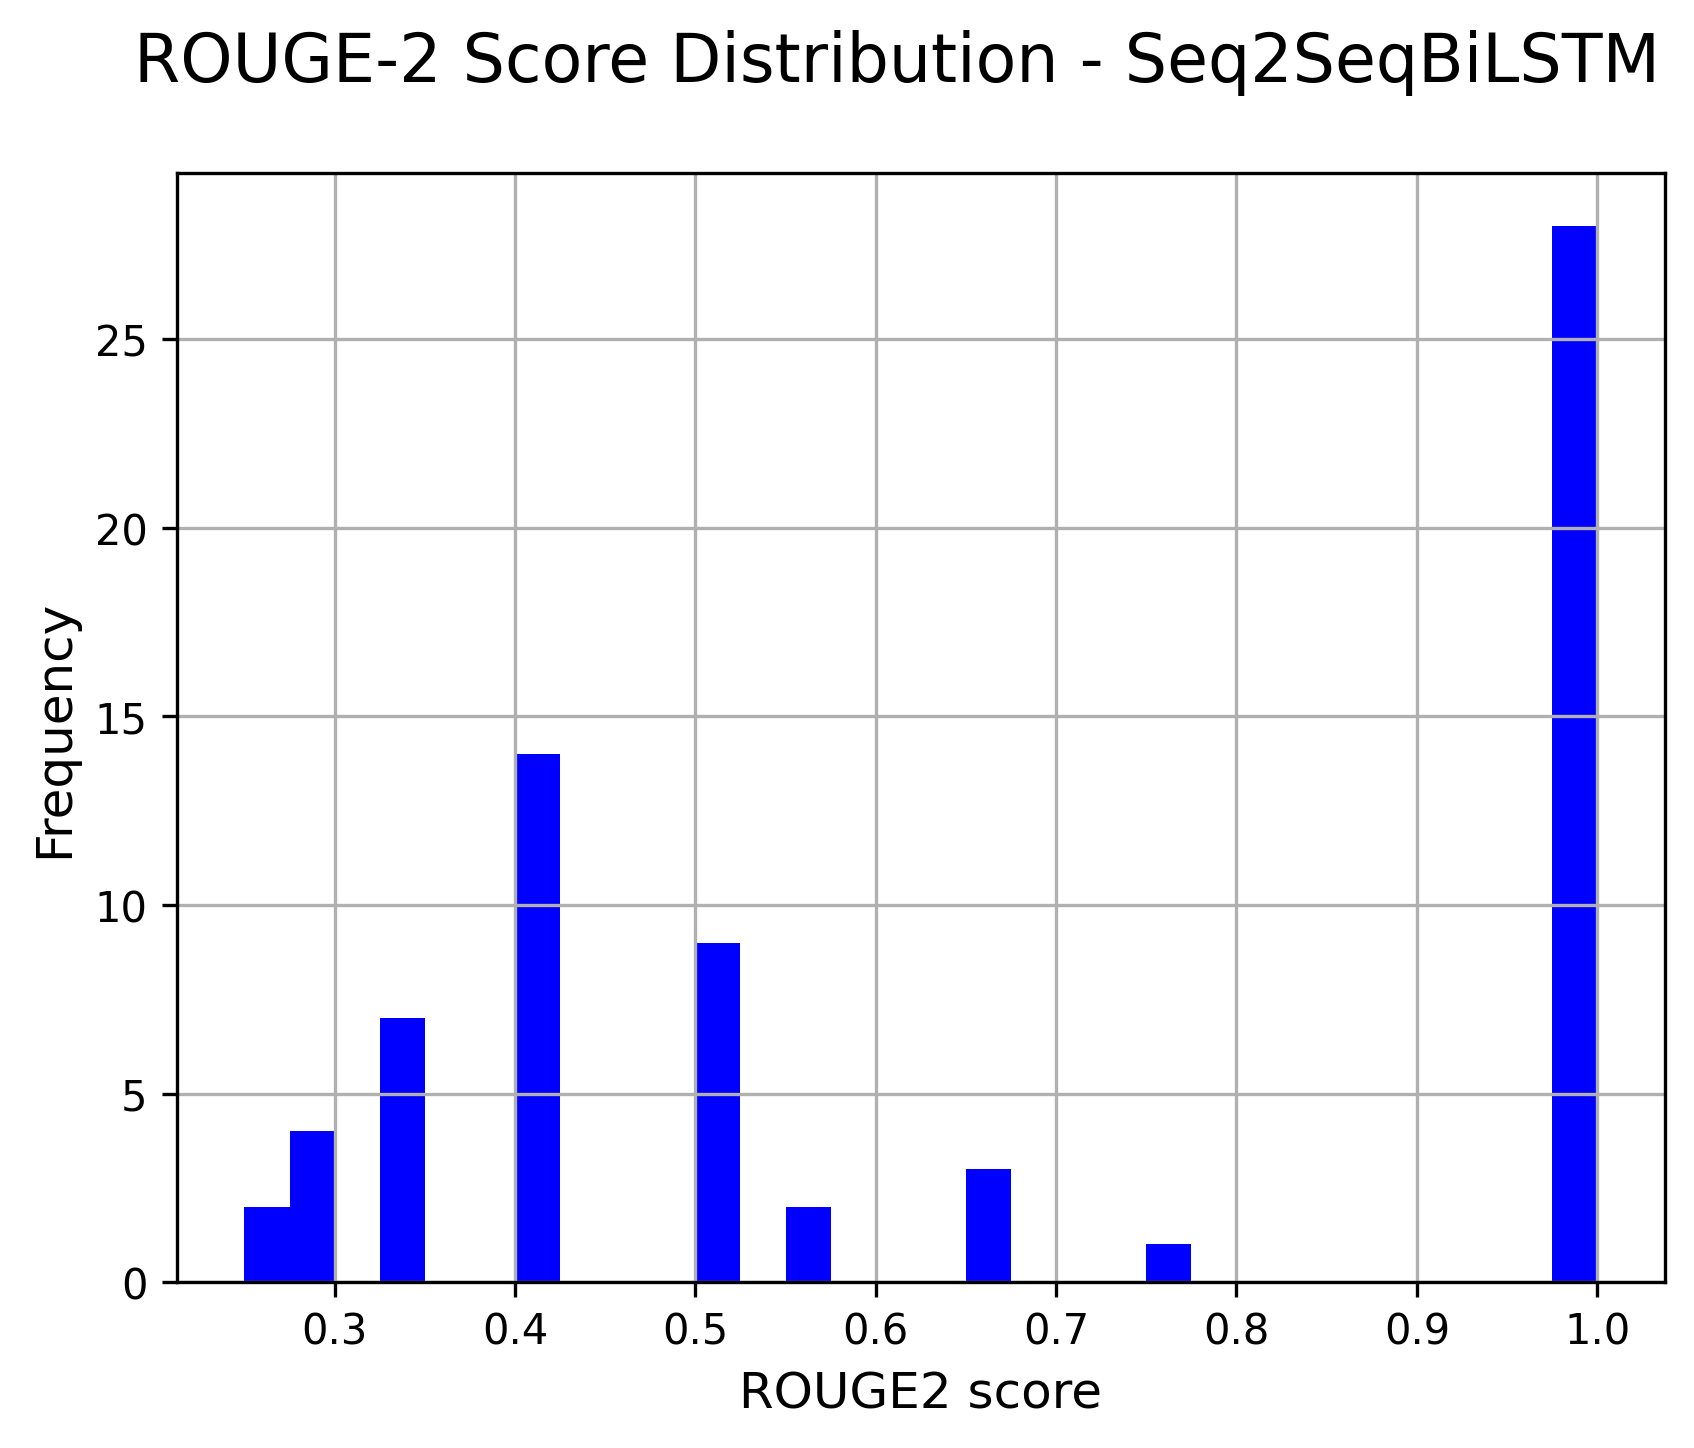
\includegraphics[width=\textwidth]{media/Seq2SeqBiLSTM_rouge2_scores.png}
        \caption{ROUGE-2 Seq2SeqBiLSTM}
    \end{subfigure}
    \hfill
    \begin{subfigure}{0.24\textwidth}
        \centering
        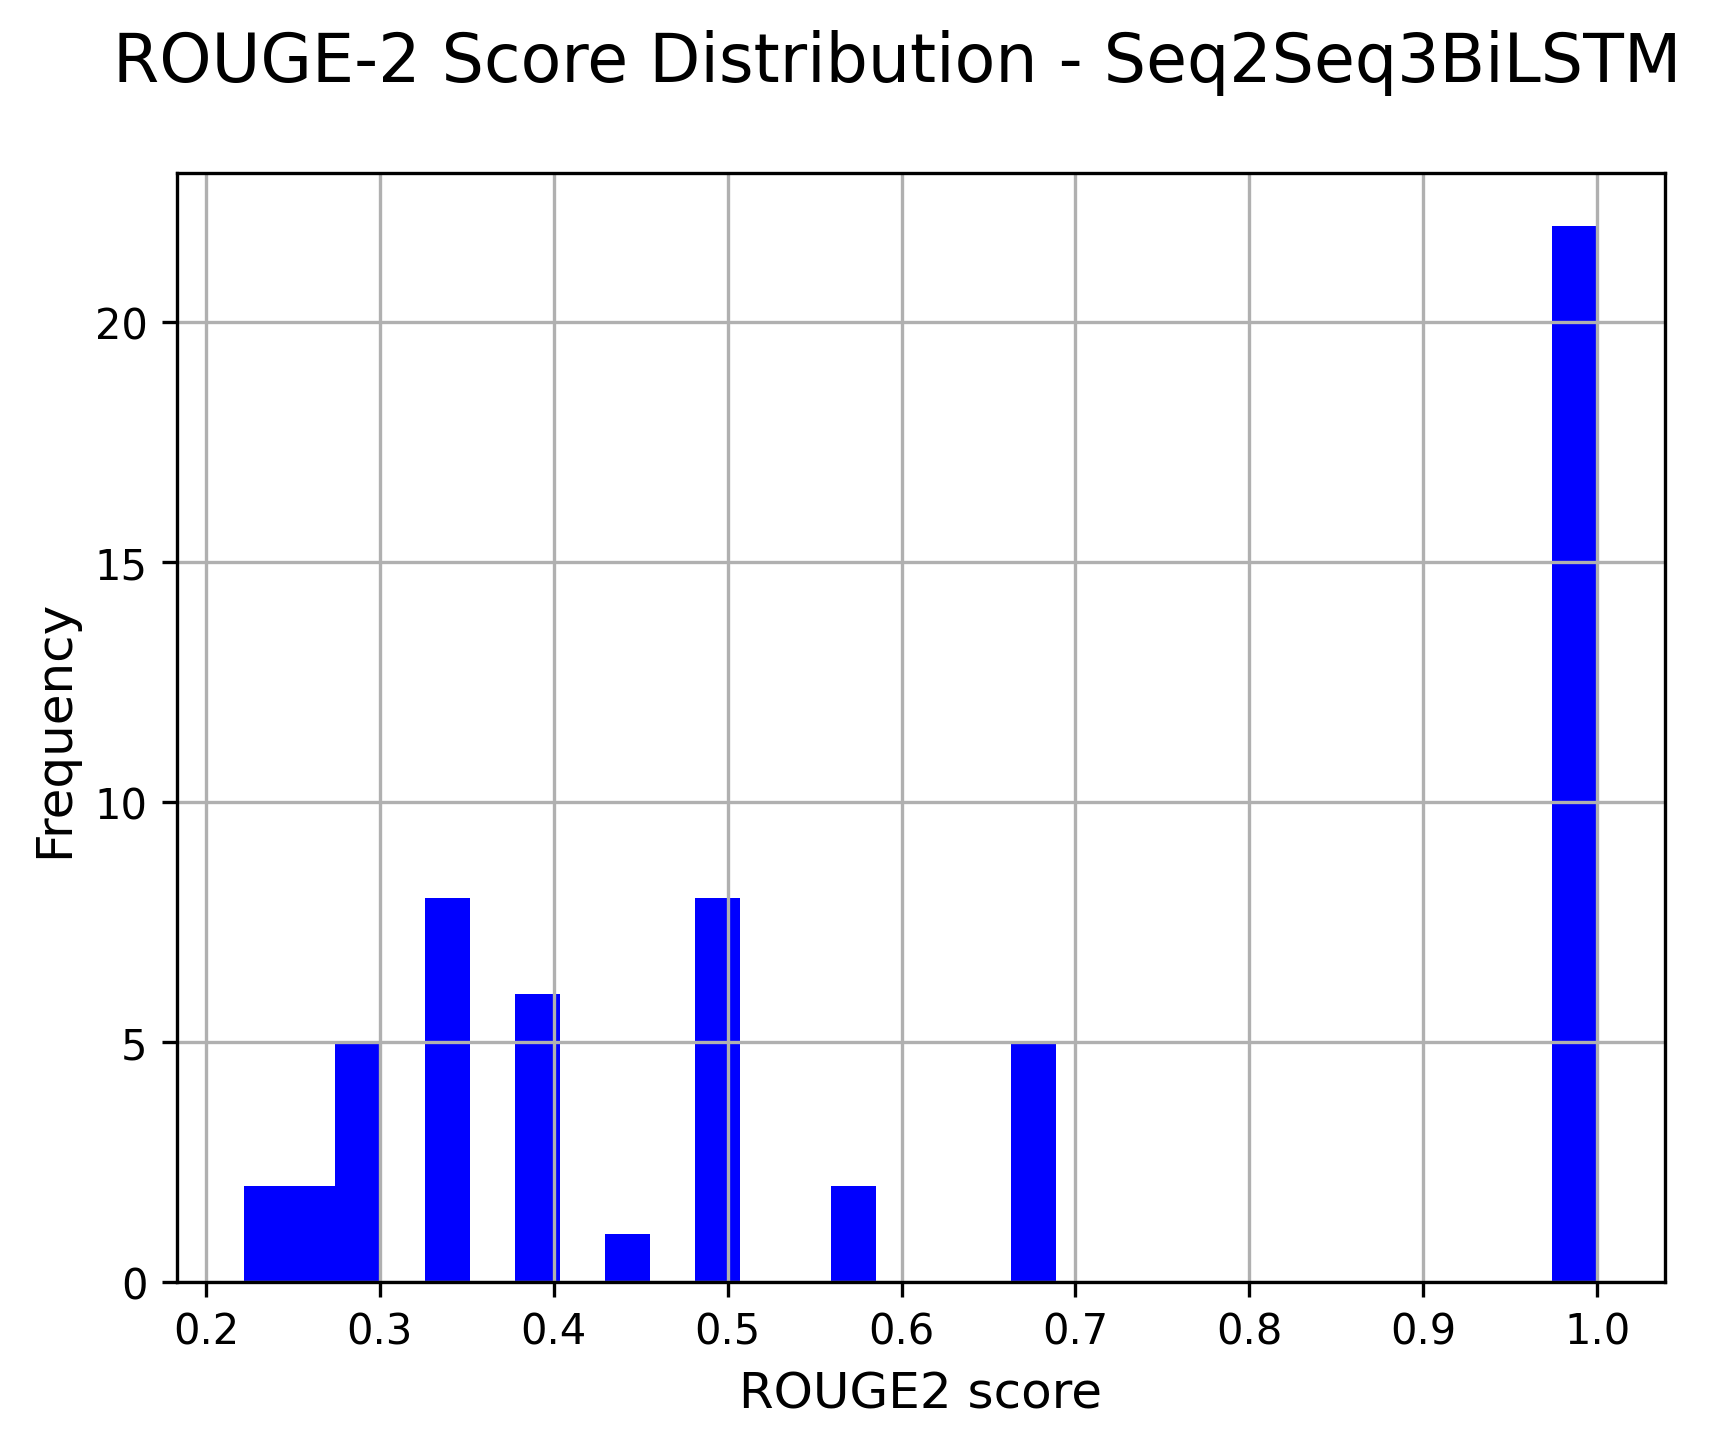
\includegraphics[width=\textwidth]{media/Seq2Seq3BiLSTM_rouge2_scores.png}
        \caption{ROUGE-2 Seq2Seq3BiLSTM}
    \end{subfigure}
    \hfill
    \begin{subfigure}{0.24\textwidth}
        \centering
        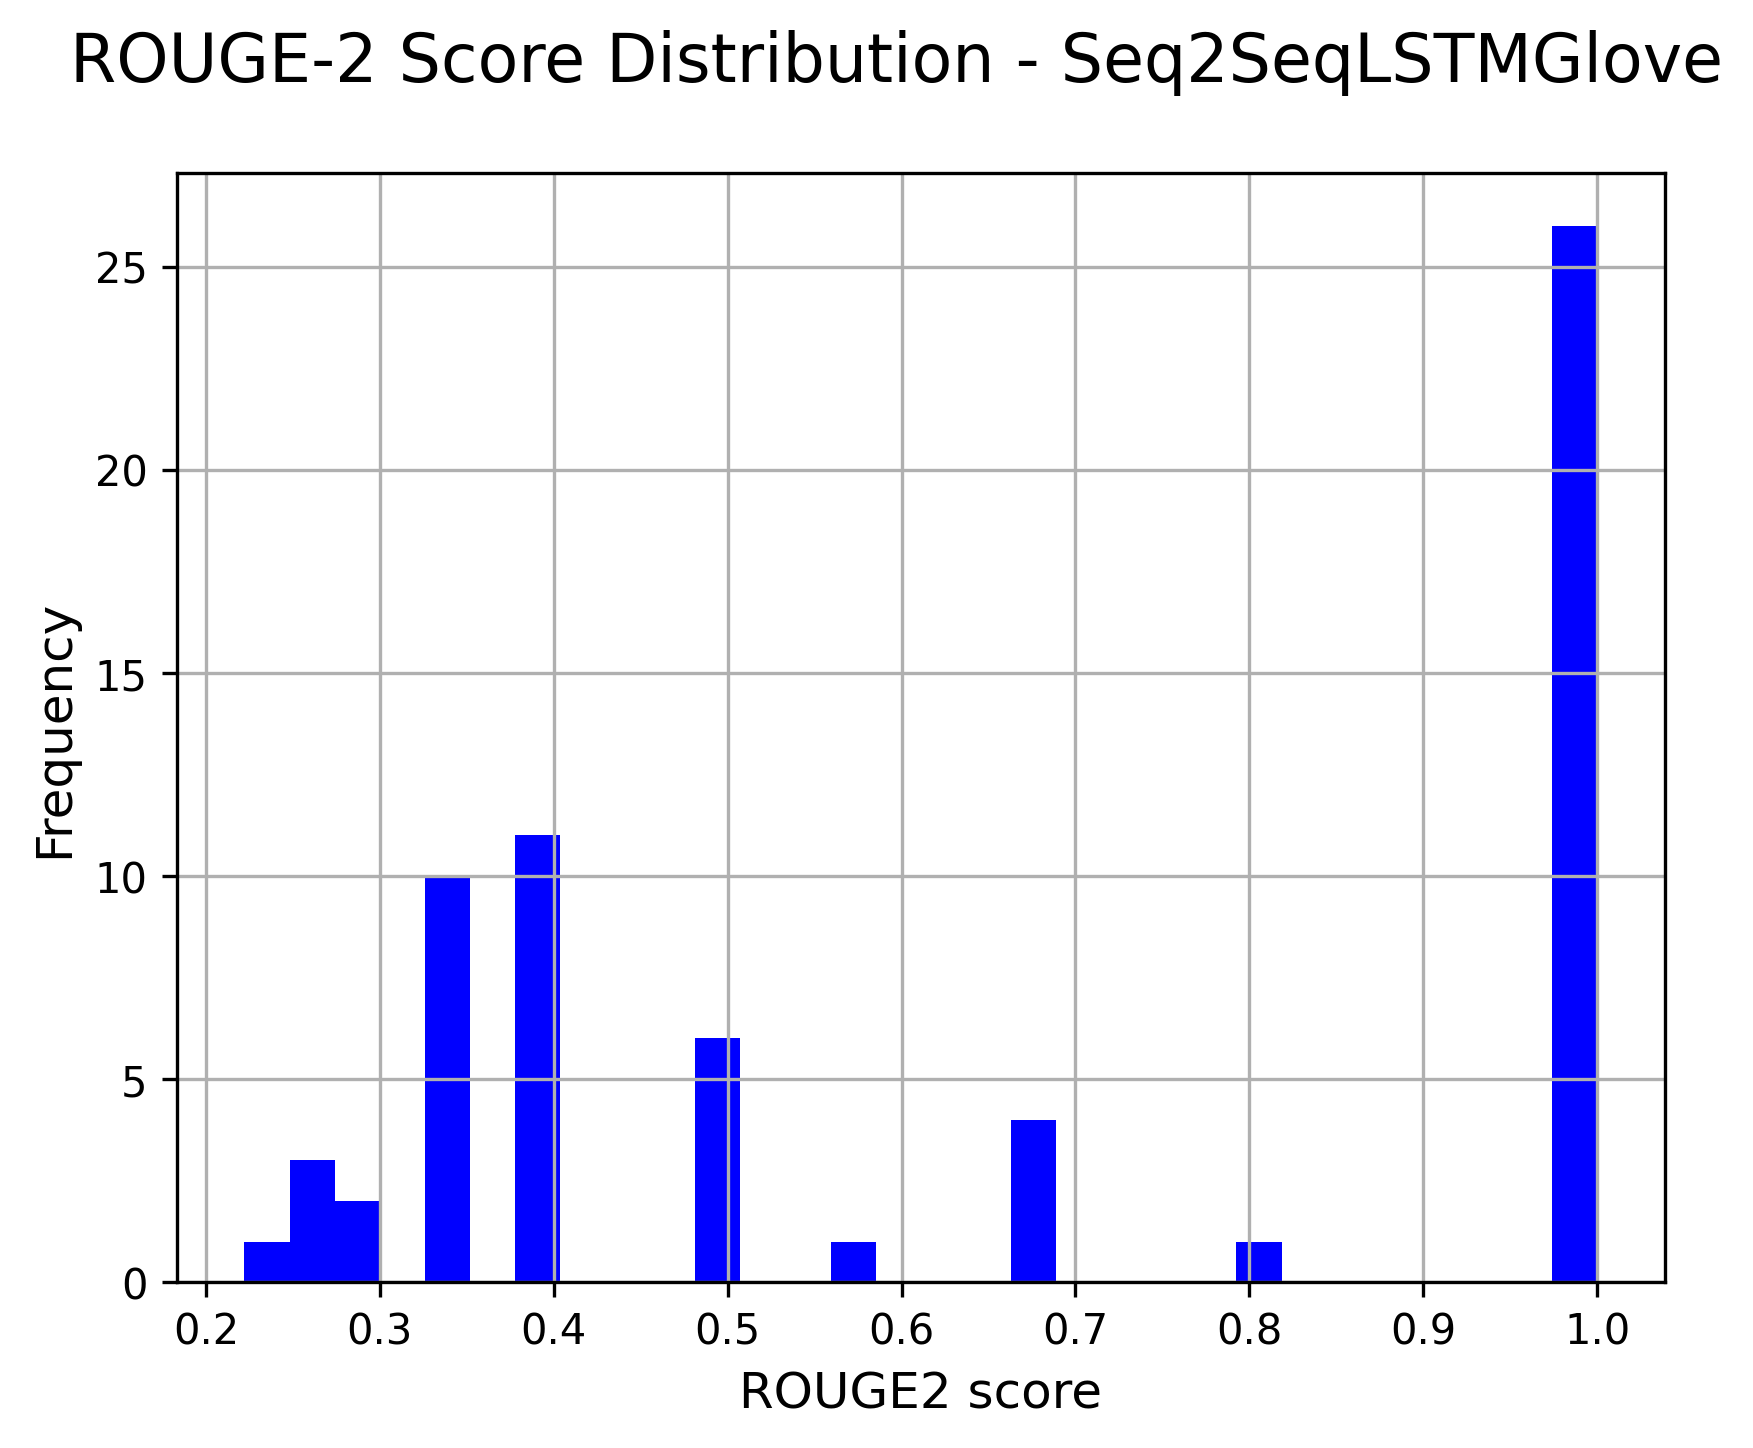
\includegraphics[width=\textwidth]{media/Seq2SeqLSTMGlove_rouge2_scores.png}
        \caption{ROUGE-2 Seq2SeqLSTMGlove}
    \end{subfigure}
    \hfill
    \begin{subfigure}{0.24\textwidth}
        \centering
        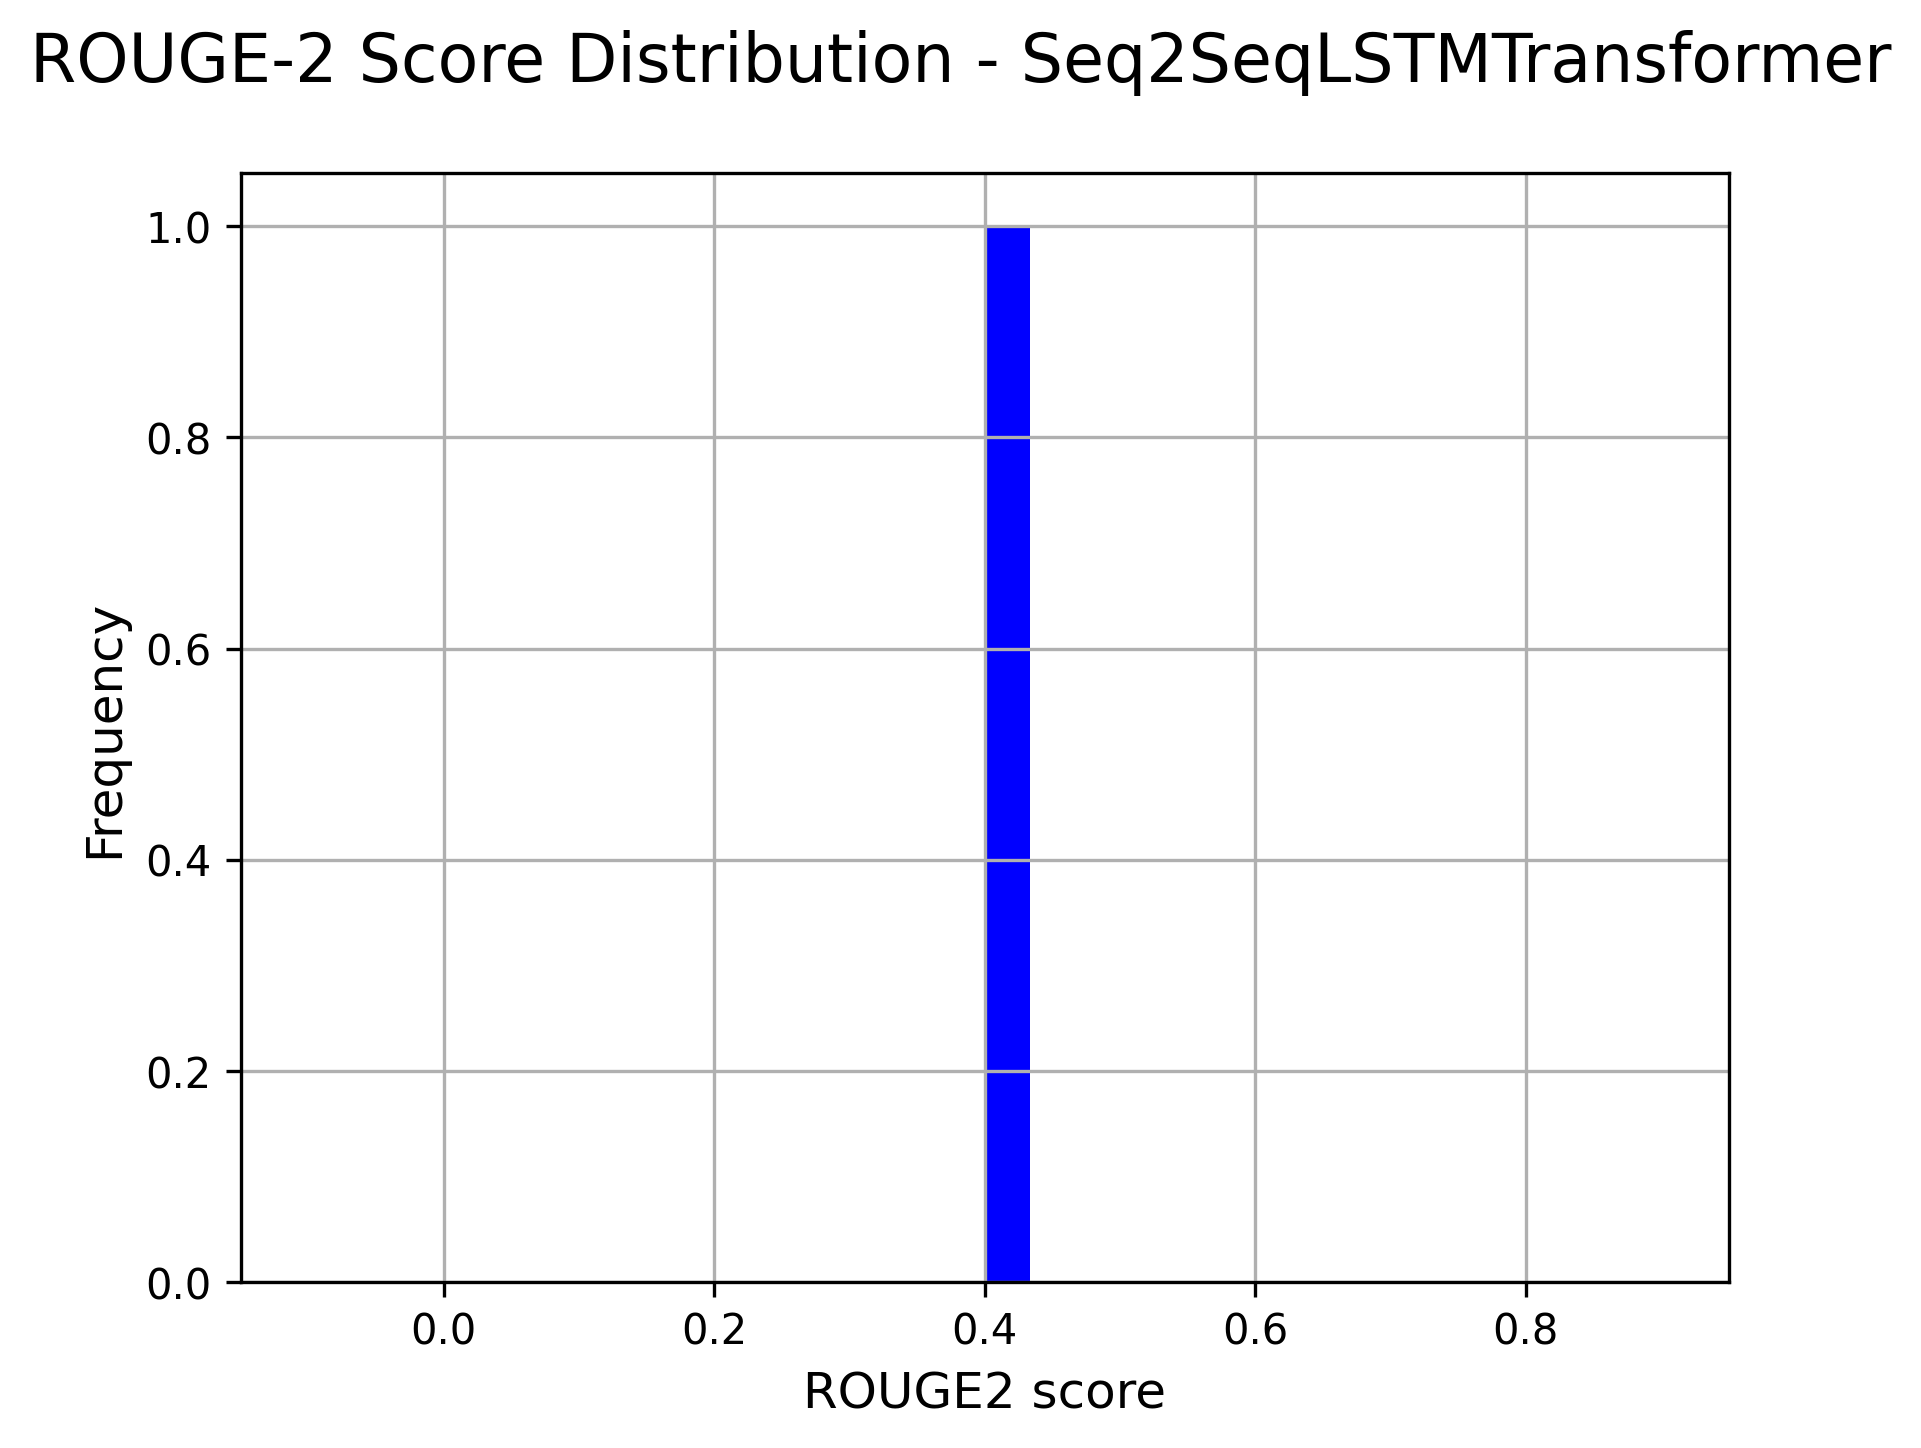
\includegraphics[width=\textwidth]{media/Seq2SeqLSTMTransformer_rouge2_scores.png}
        \caption{ROUGE-2 Seq2SeqLSTMTransformer}
    \end{subfigure}

    \begin{subfigure}{0.24\textwidth}
        \centering
        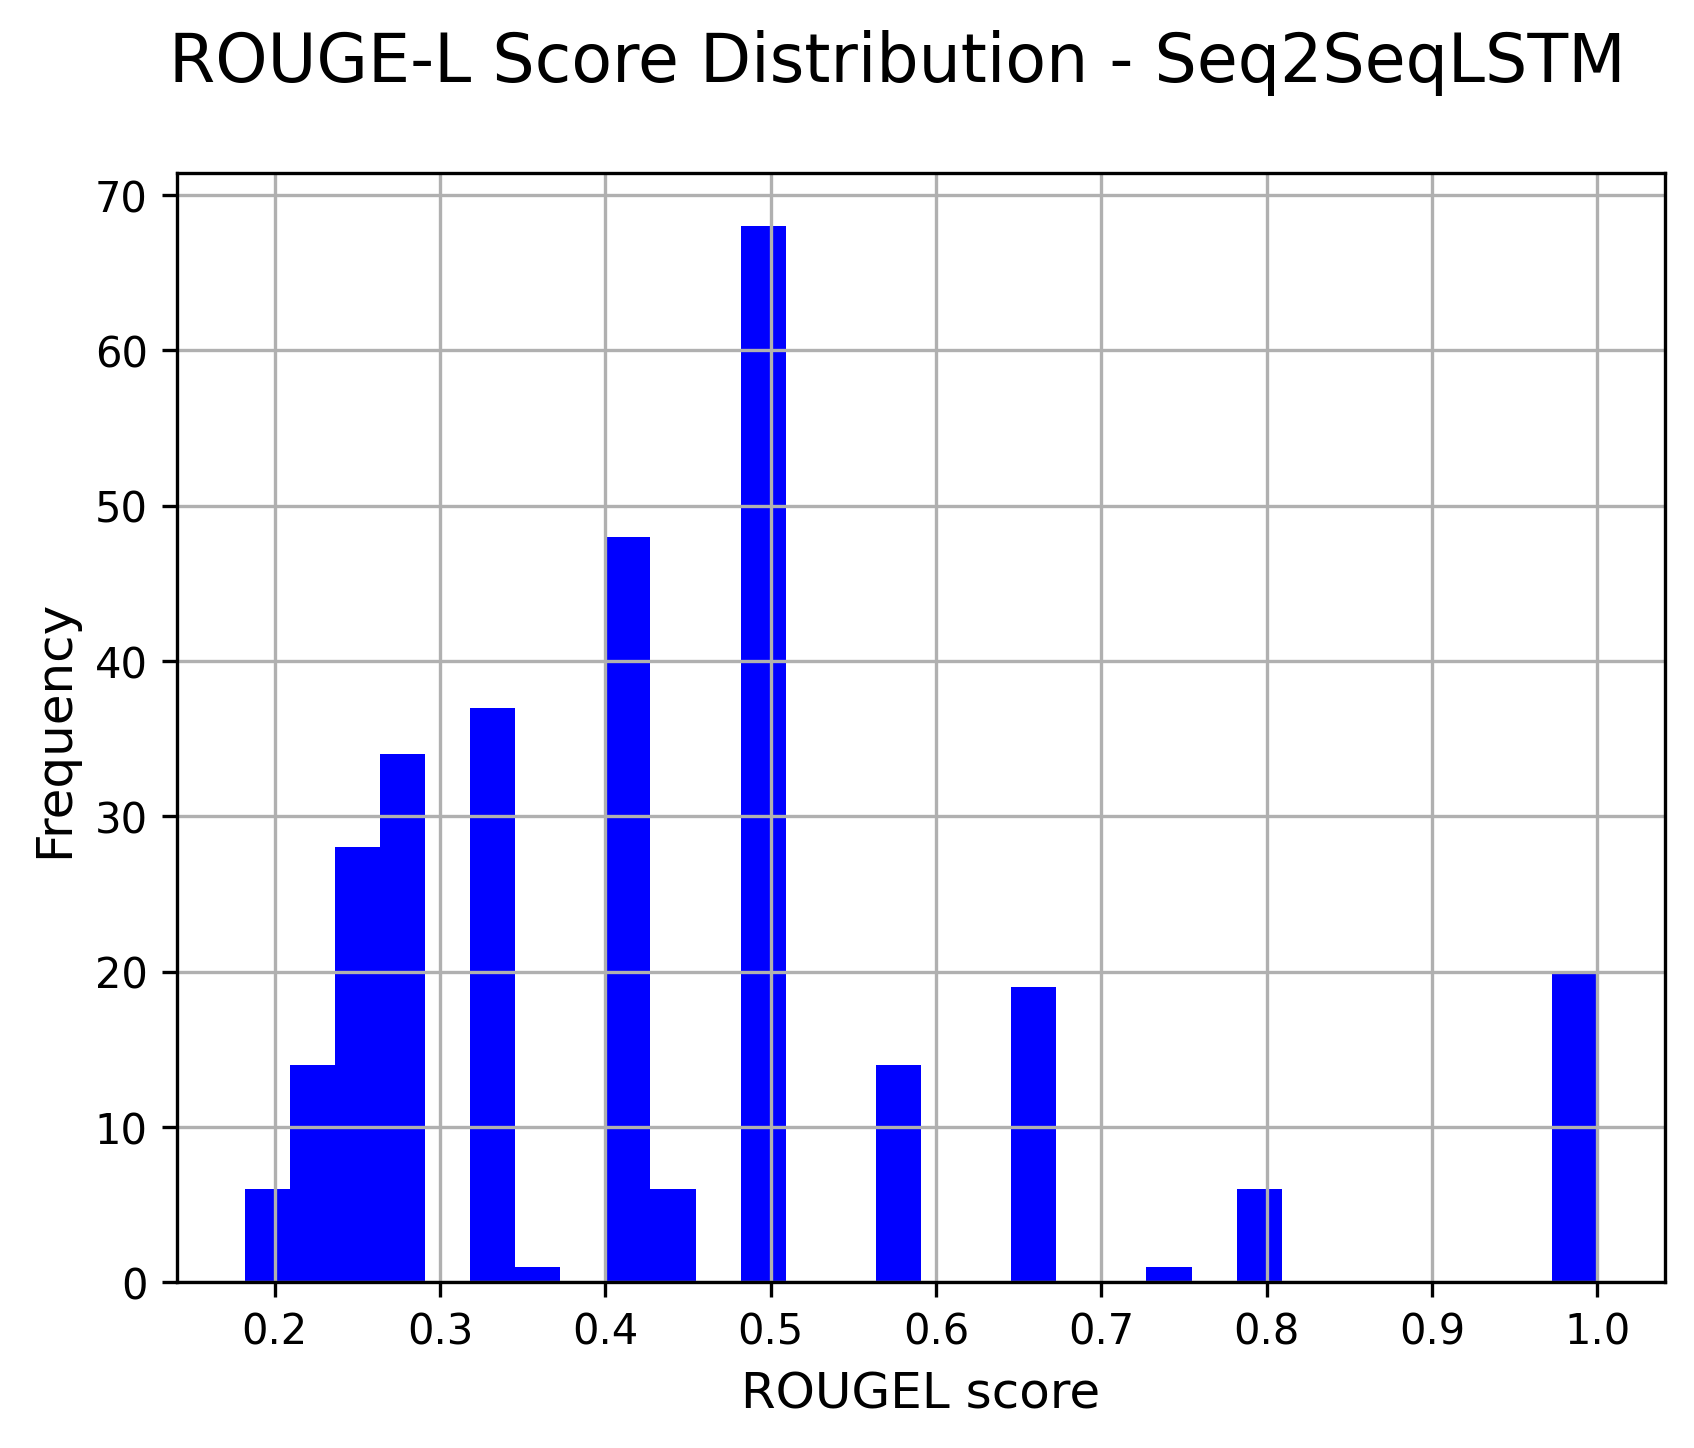
\includegraphics[width=\textwidth]{media/Seq2SeqLSTM_rougeL_scores.png}
        \caption{ROUGE-L Seq2SeqLSTM}
    \end{subfigure}
    \hfill
    \begin{subfigure}{0.24\textwidth}
        \centering
        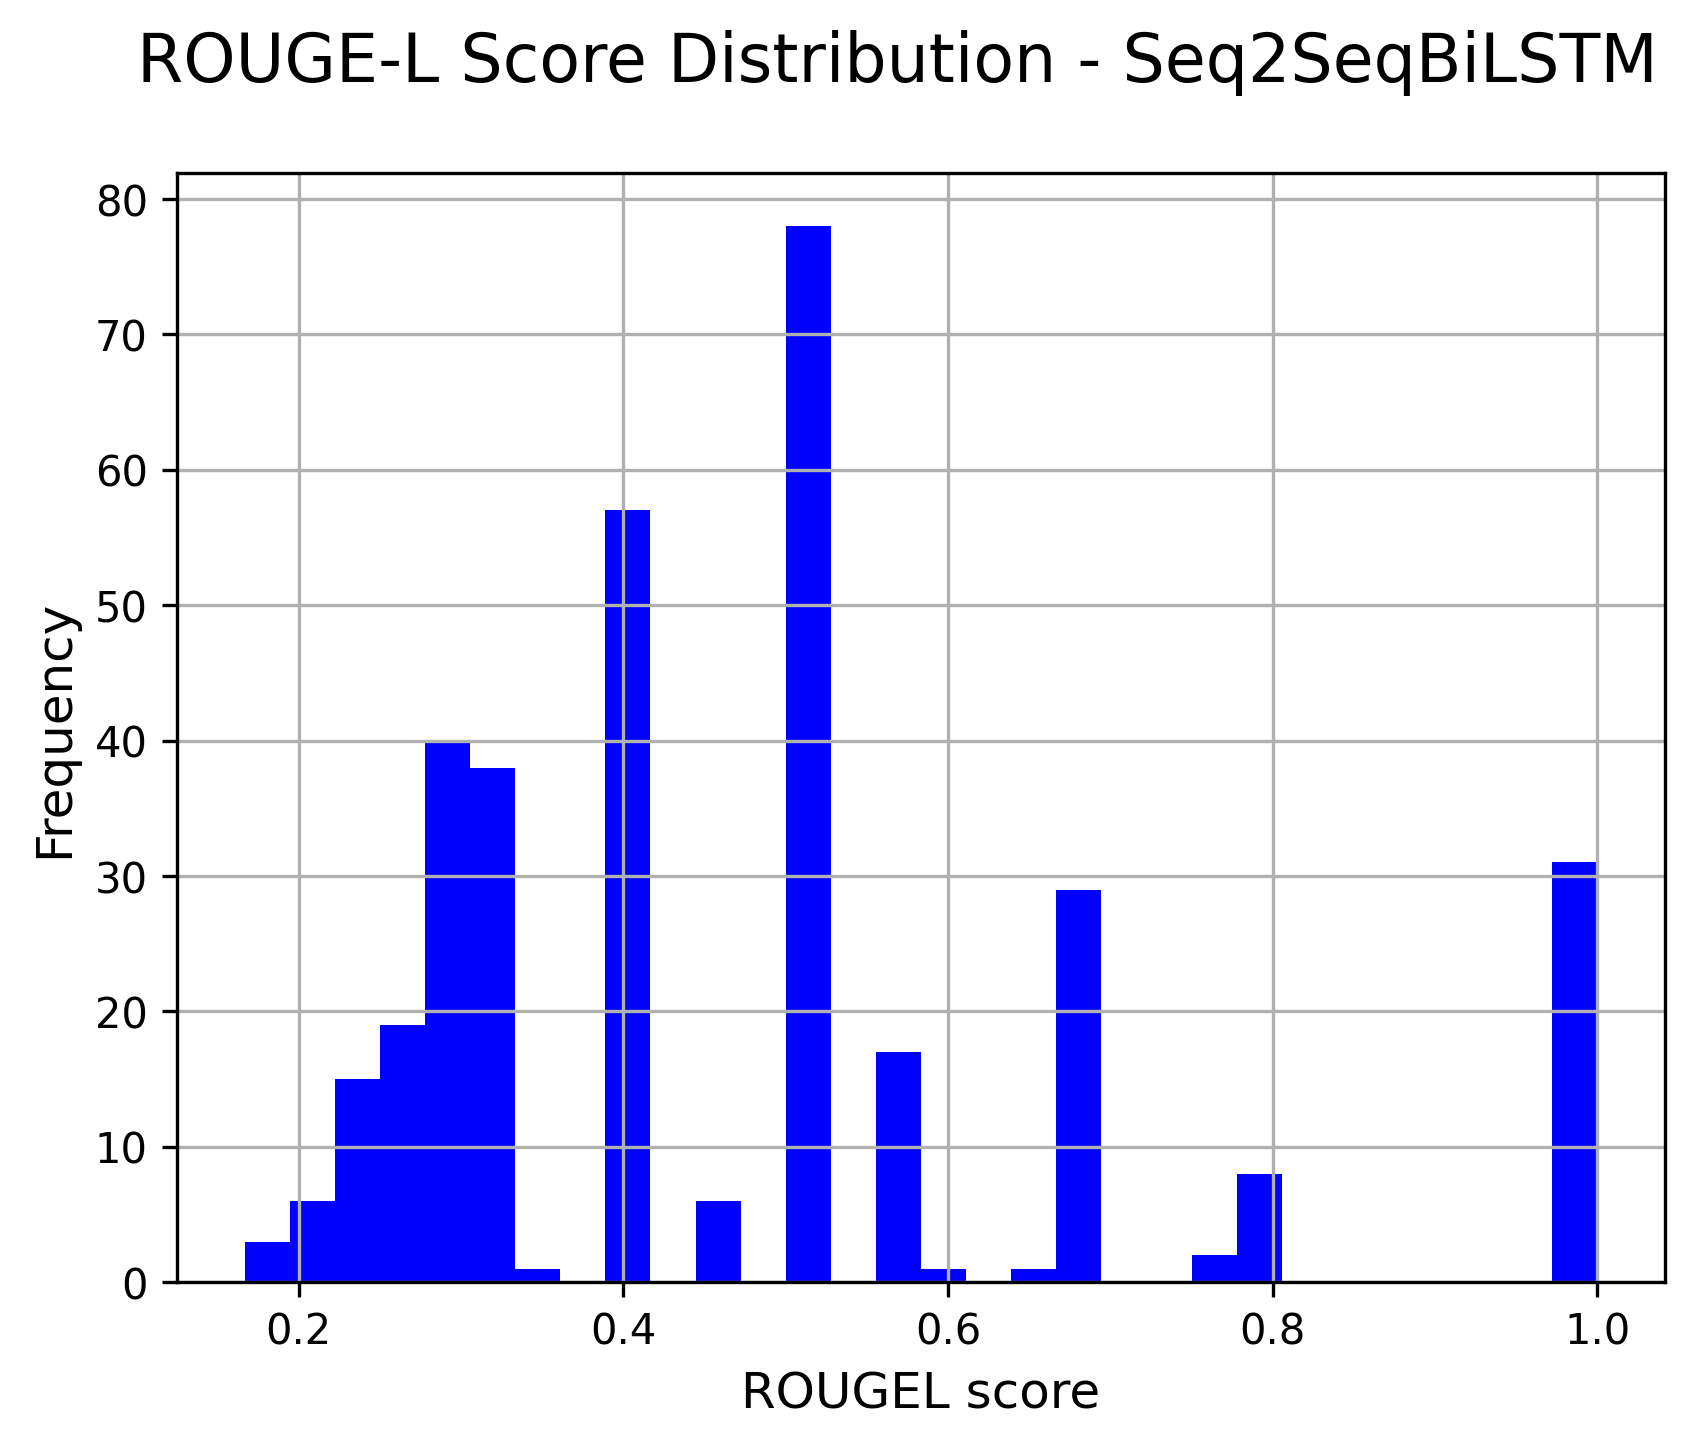
\includegraphics[width=\textwidth]{media/Seq2SeqBiLSTM_rougeL_scores.png}
        \caption{ROUGE-L Seq2SeqBiLSTM}
    \end{subfigure}
    \hfill
    \begin{subfigure}{0.24\textwidth}
        \centering
        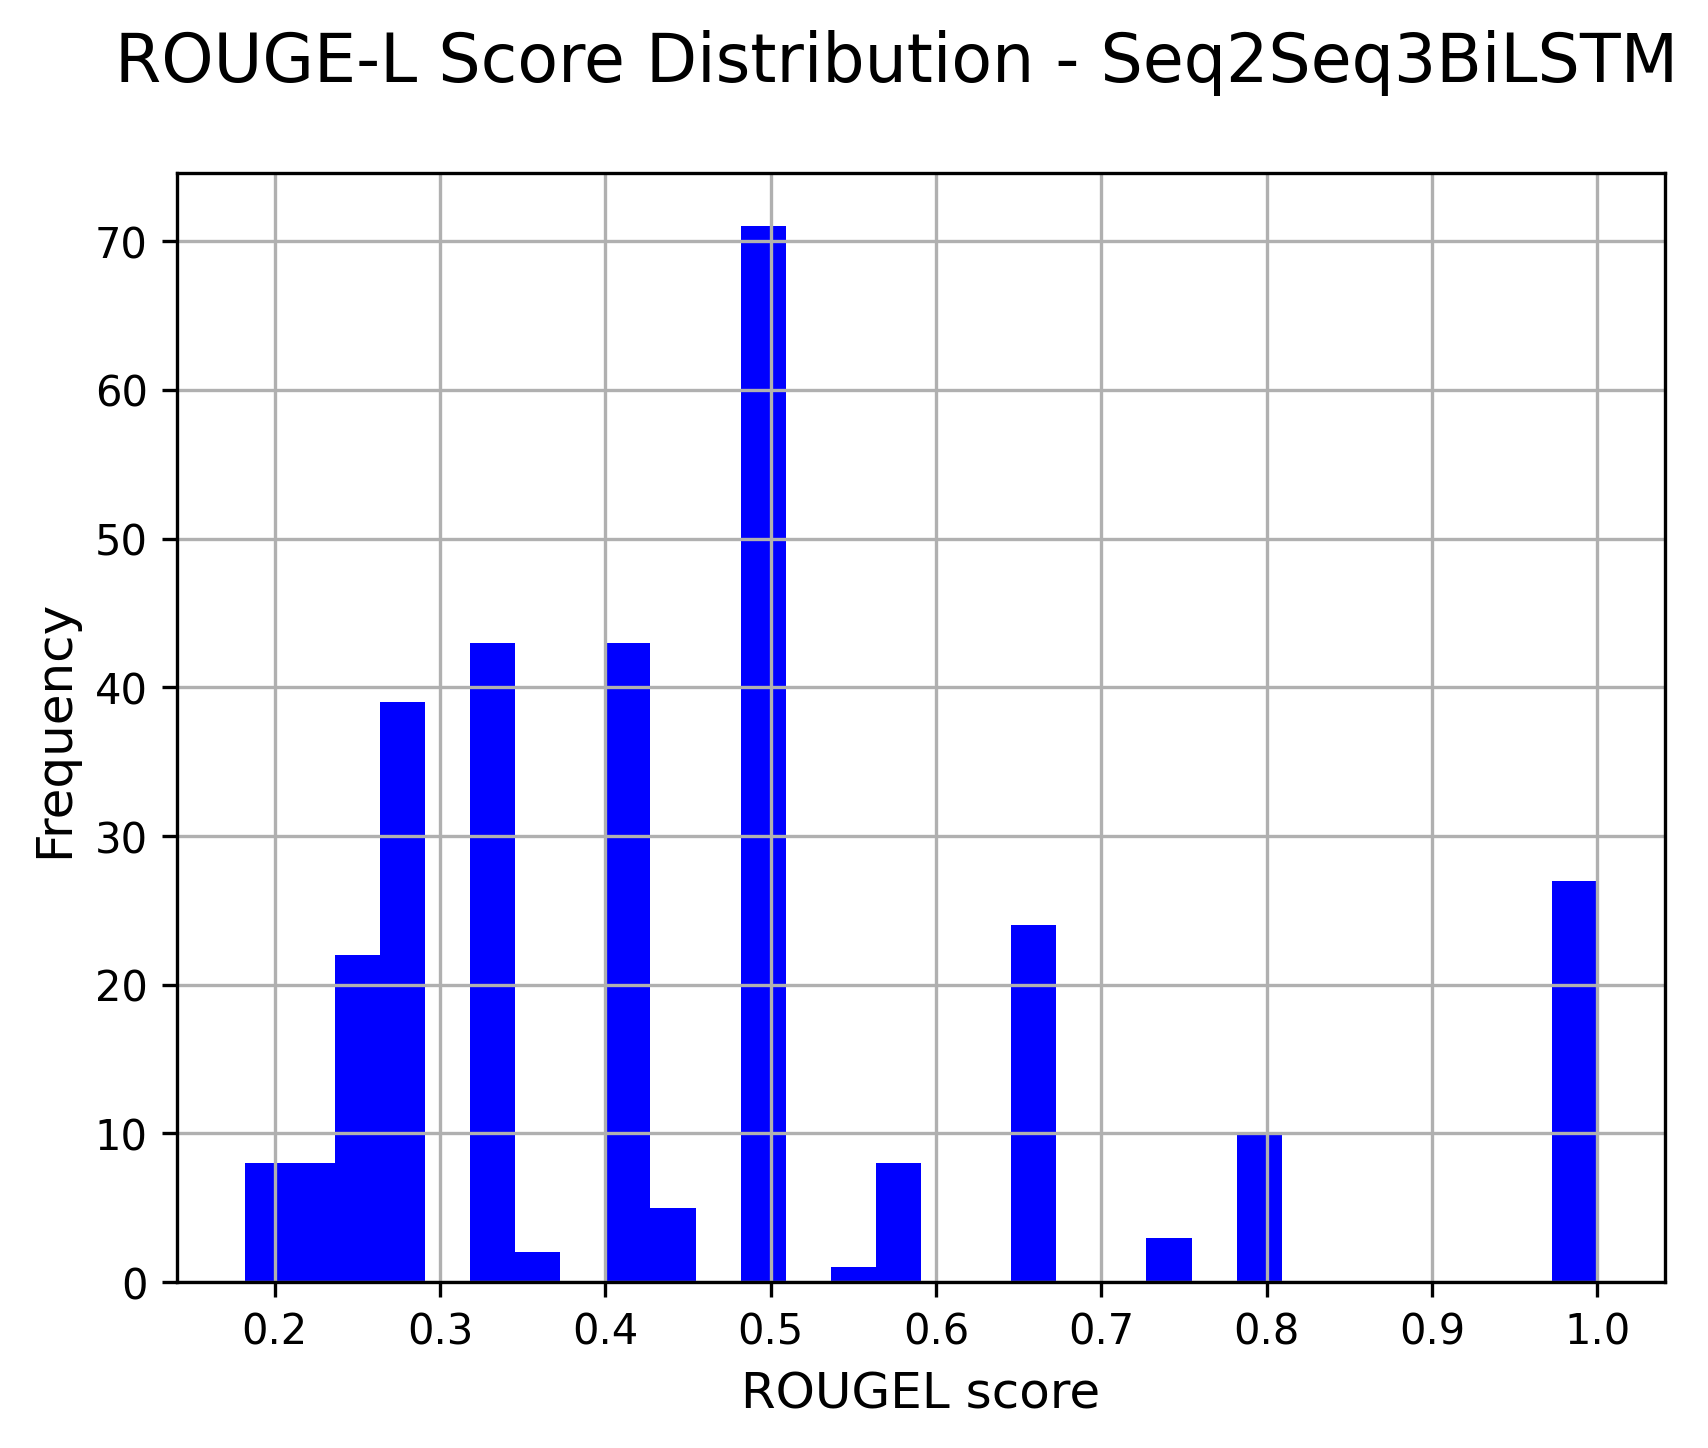
\includegraphics[width=\textwidth]{media/Seq2Seq3BiLSTM_rougeL_scores.png}
        \caption{ROUGE-L Seq2Seq3BiLSTM}
    \end{subfigure}
    \hfill
    \begin{subfigure}{0.24\textwidth}
        \centering
        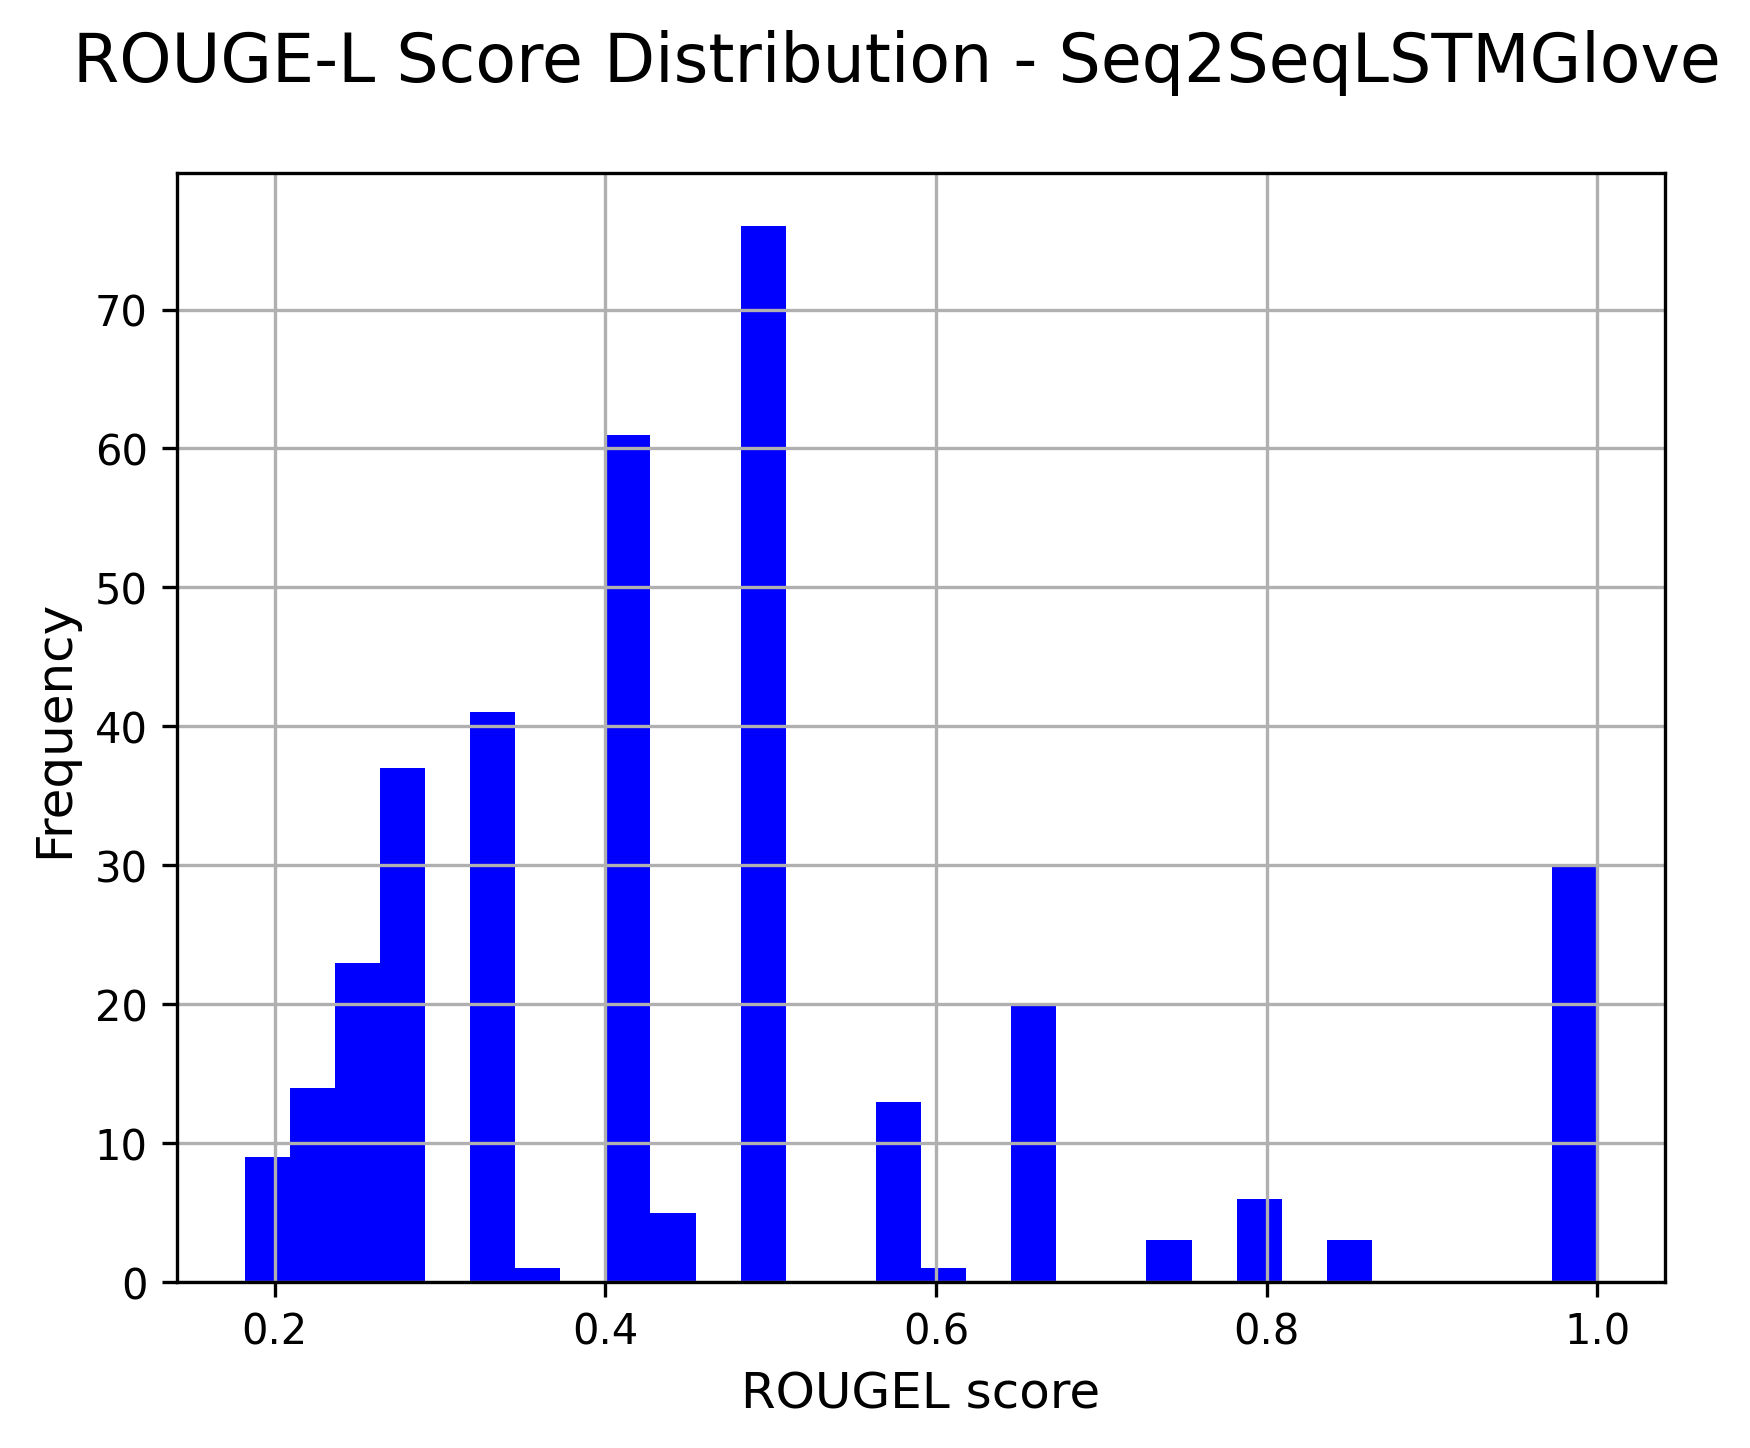
\includegraphics[width=\textwidth]{media/Seq2SeqLSTMGlove_rougeL_scores.png}
        \caption{ROUGE-L Seq2SeqLSTMGlove}
    \end{subfigure}
    \hfill
    \begin{subfigure}{0.24\textwidth}
        \centering
        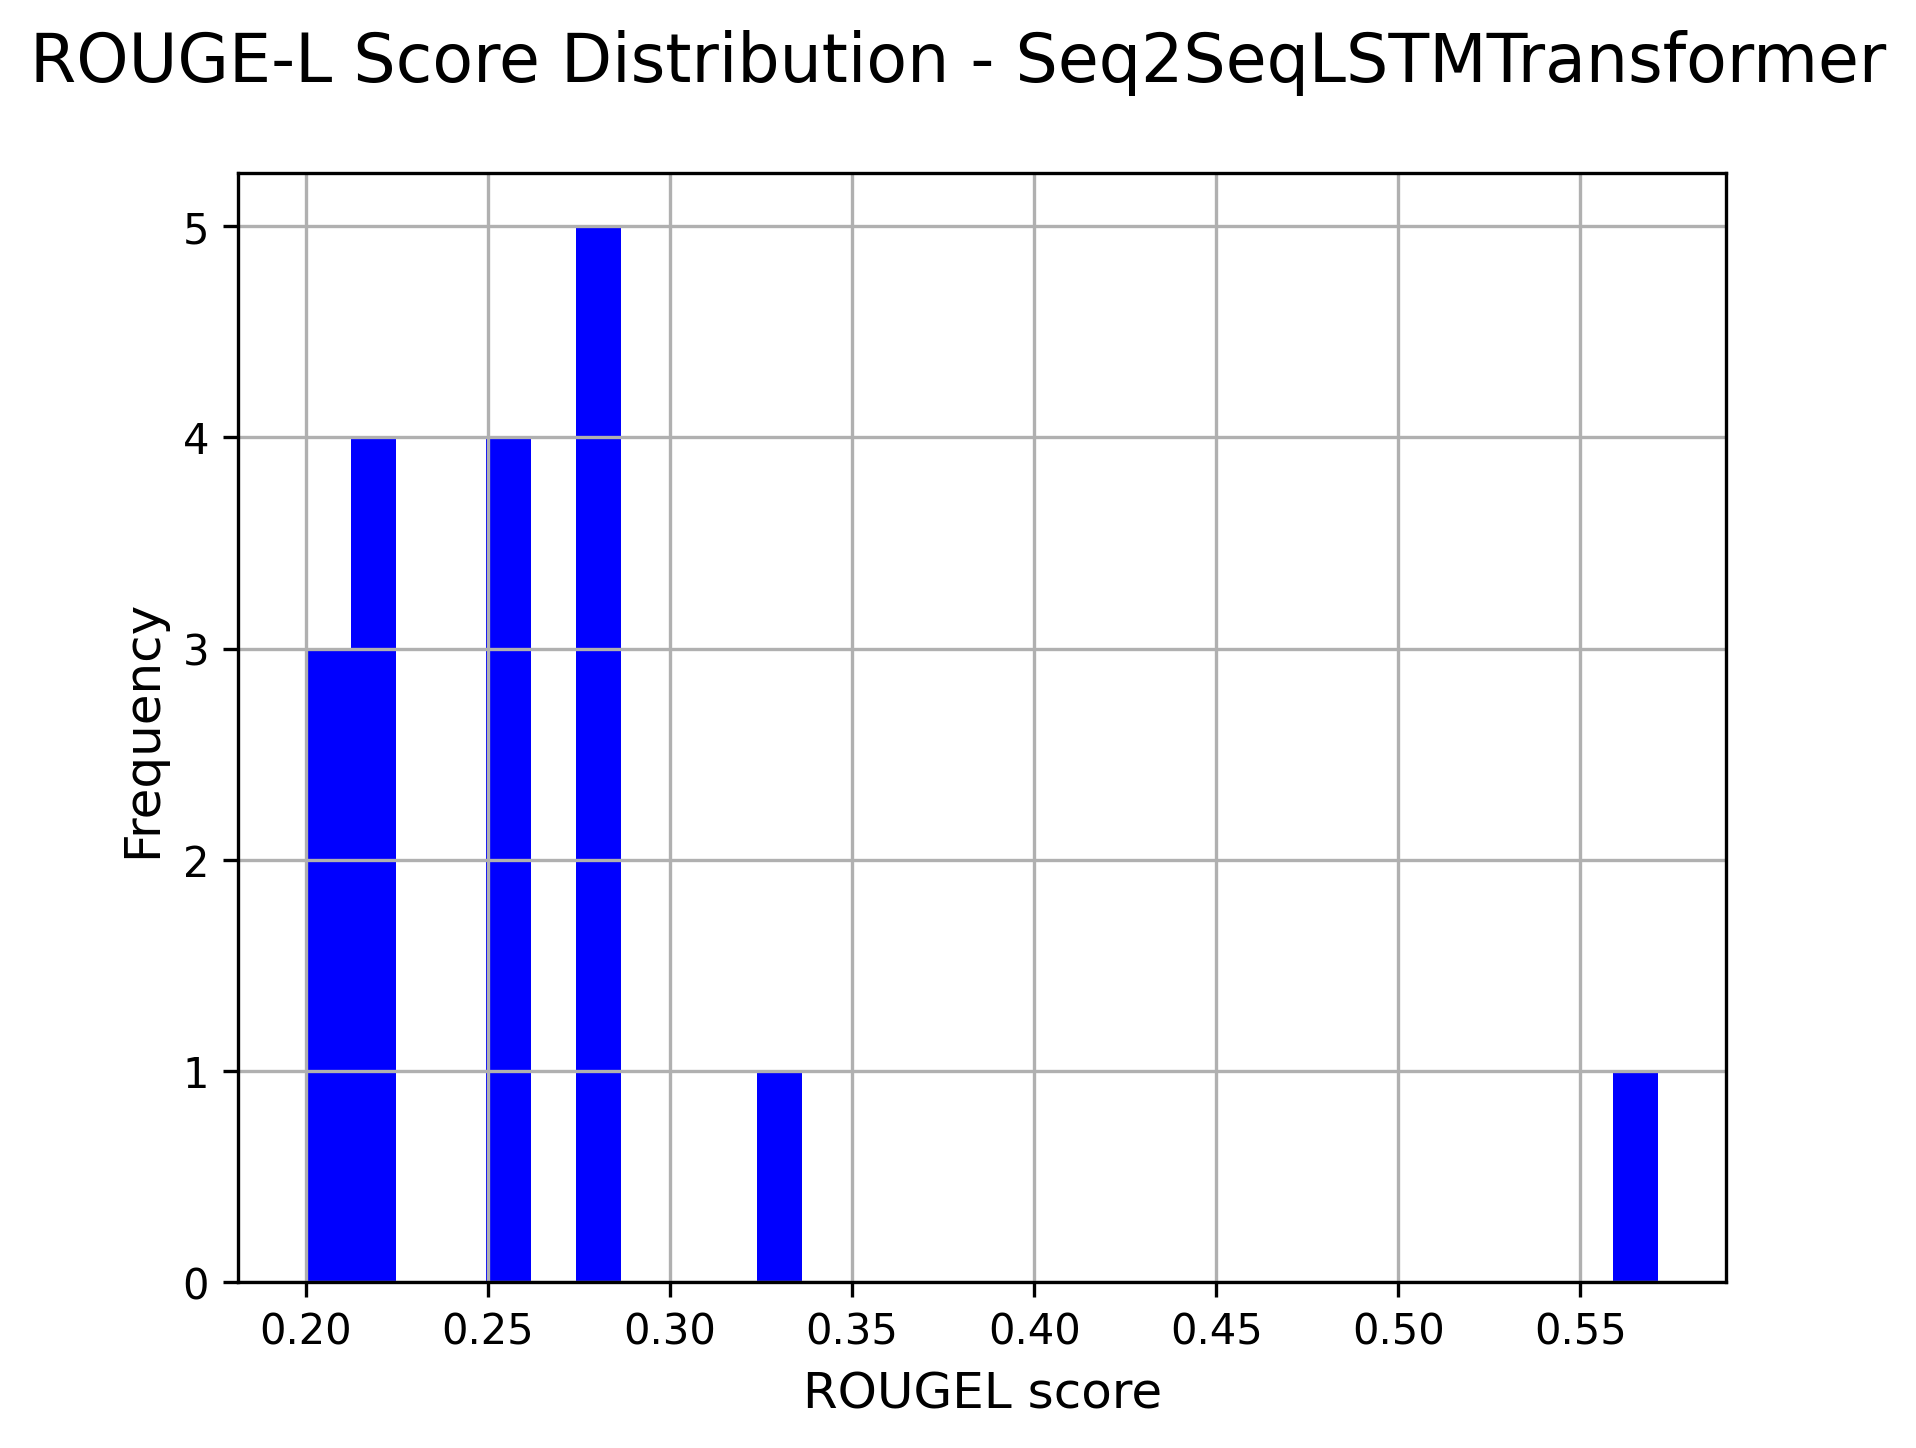
\includegraphics[width=\textwidth]{media/Seq2SeqLSTMTransformer_rougeL_scores.png}
        \caption{ROUGE-L Seq2SeqLSTMTransformer}
    \end{subfigure}

    \caption{Confronto dei punteggi ROUGE tra i modelli Seq2SeqLSTM, Seq2SeqBiLSTM, Seq2Seq3BiLSTM, Seq2SeqLSTMGlove e Seq2SeqLSTMTransformer.}
    \label{fig:rouge_comparison}
\end{figure}

\subsection{WER (Word Error Rate)}
Il WER \`e una metrica che calcola il tasso di errore tra due sequenze di parole.\\
In particolare, il WER calcola il numero di operazioni di inserimento, cancellazione e sostituzione necessarie per trasformare una sequenza di parole in un'altra.\\

Il confronto del WER, mostrato nella Figura \ref{fig:wer_comparison}, evidenzia che il modello Seq2SeqBiLSTM ottiene risultati migliori, indicando una maggiore accuratezza nella generazione delle parole.

\begin{figure}[H]
    \centering
    \begin{subfigure}{0.22\textwidth}
        \centering
        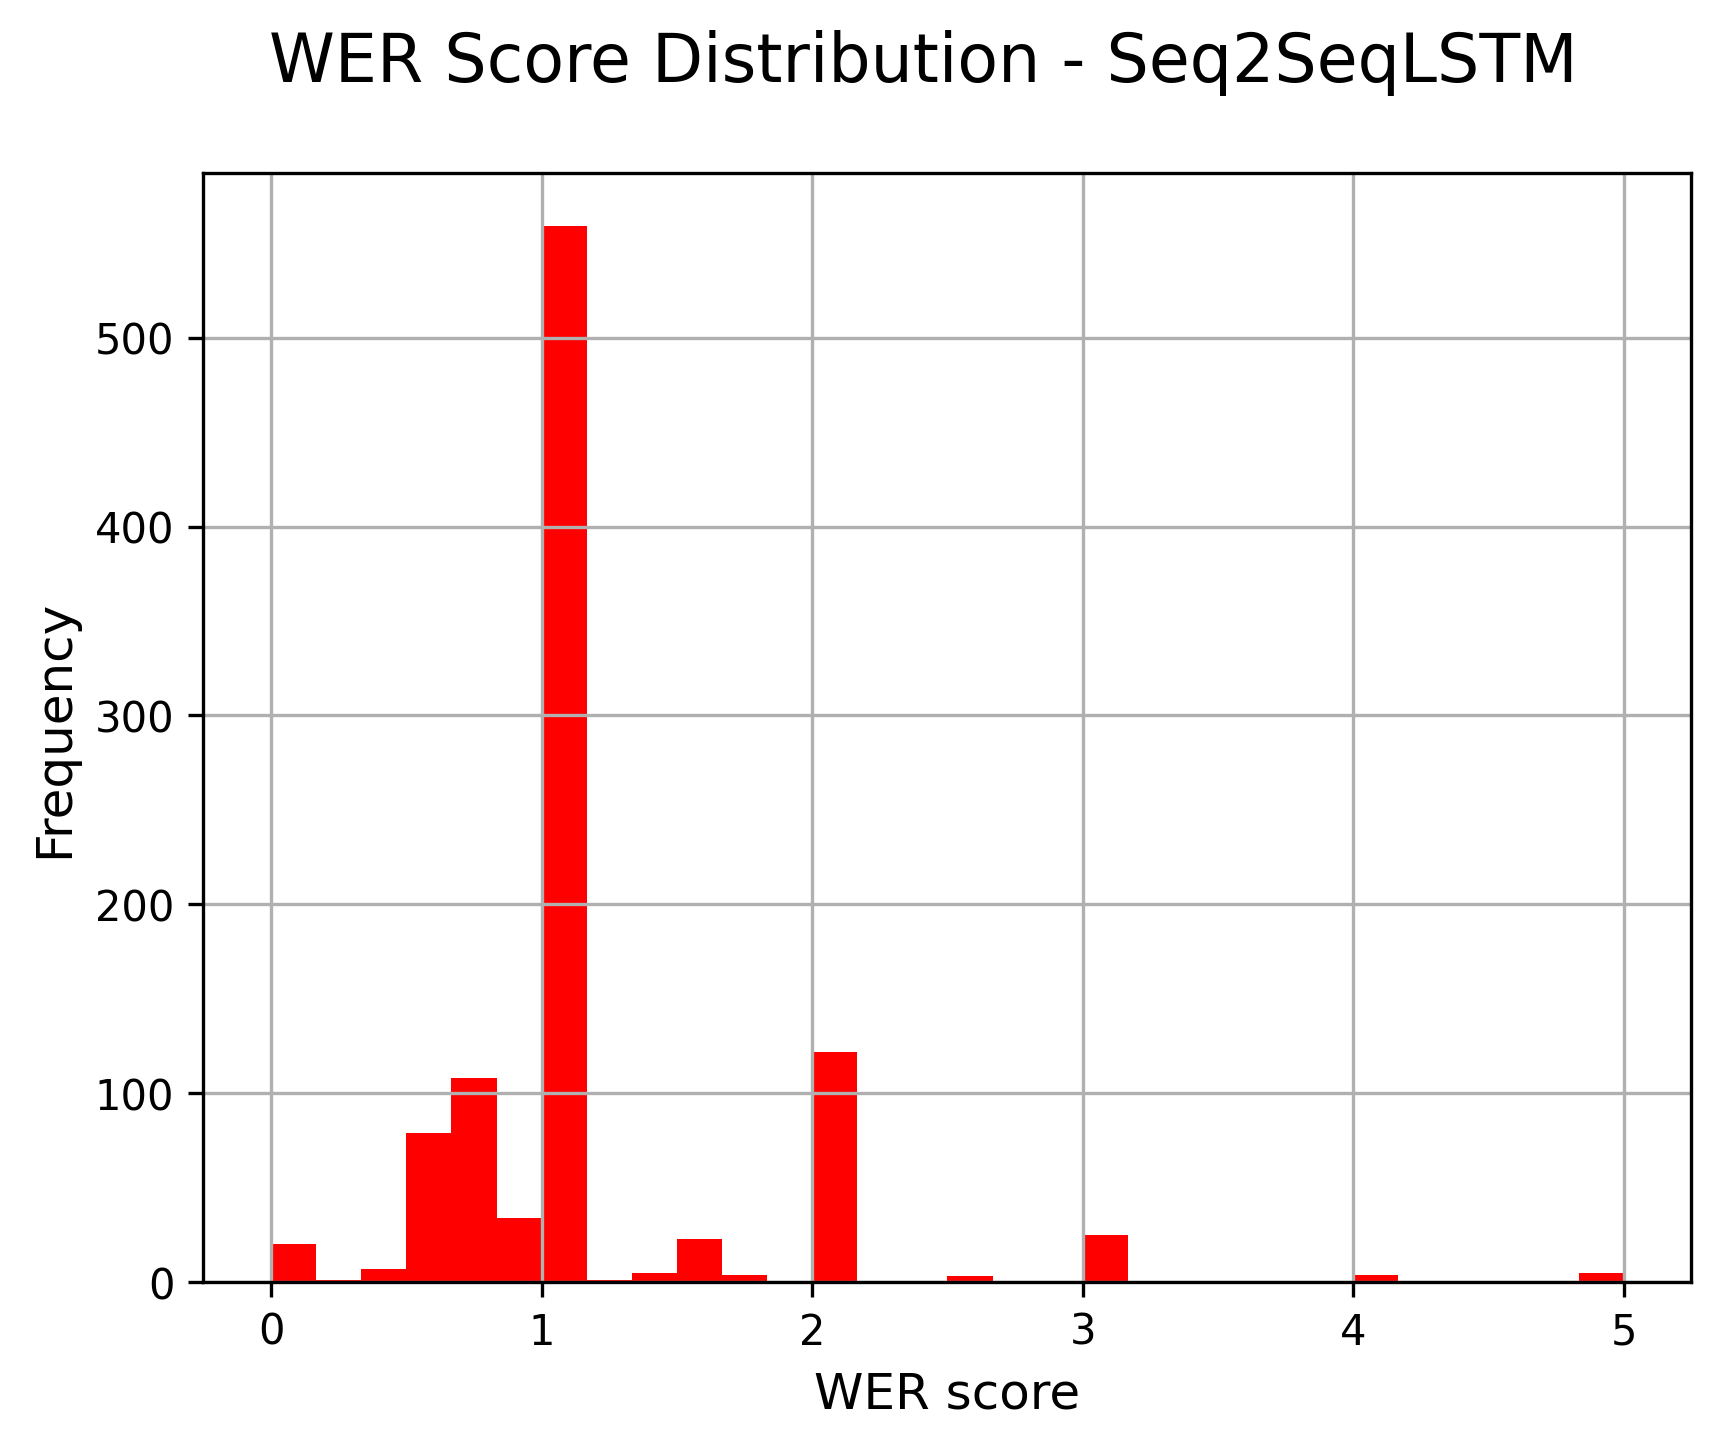
\includegraphics[width=\textwidth]{media/Seq2SeqLSTM_wer_scores.png}
        \caption{WER Seq2SeqLSTM. Valore medio: 1.1254}
    \end{subfigure}
    \hfill
    \begin{subfigure}{0.22\textwidth}
        \centering
        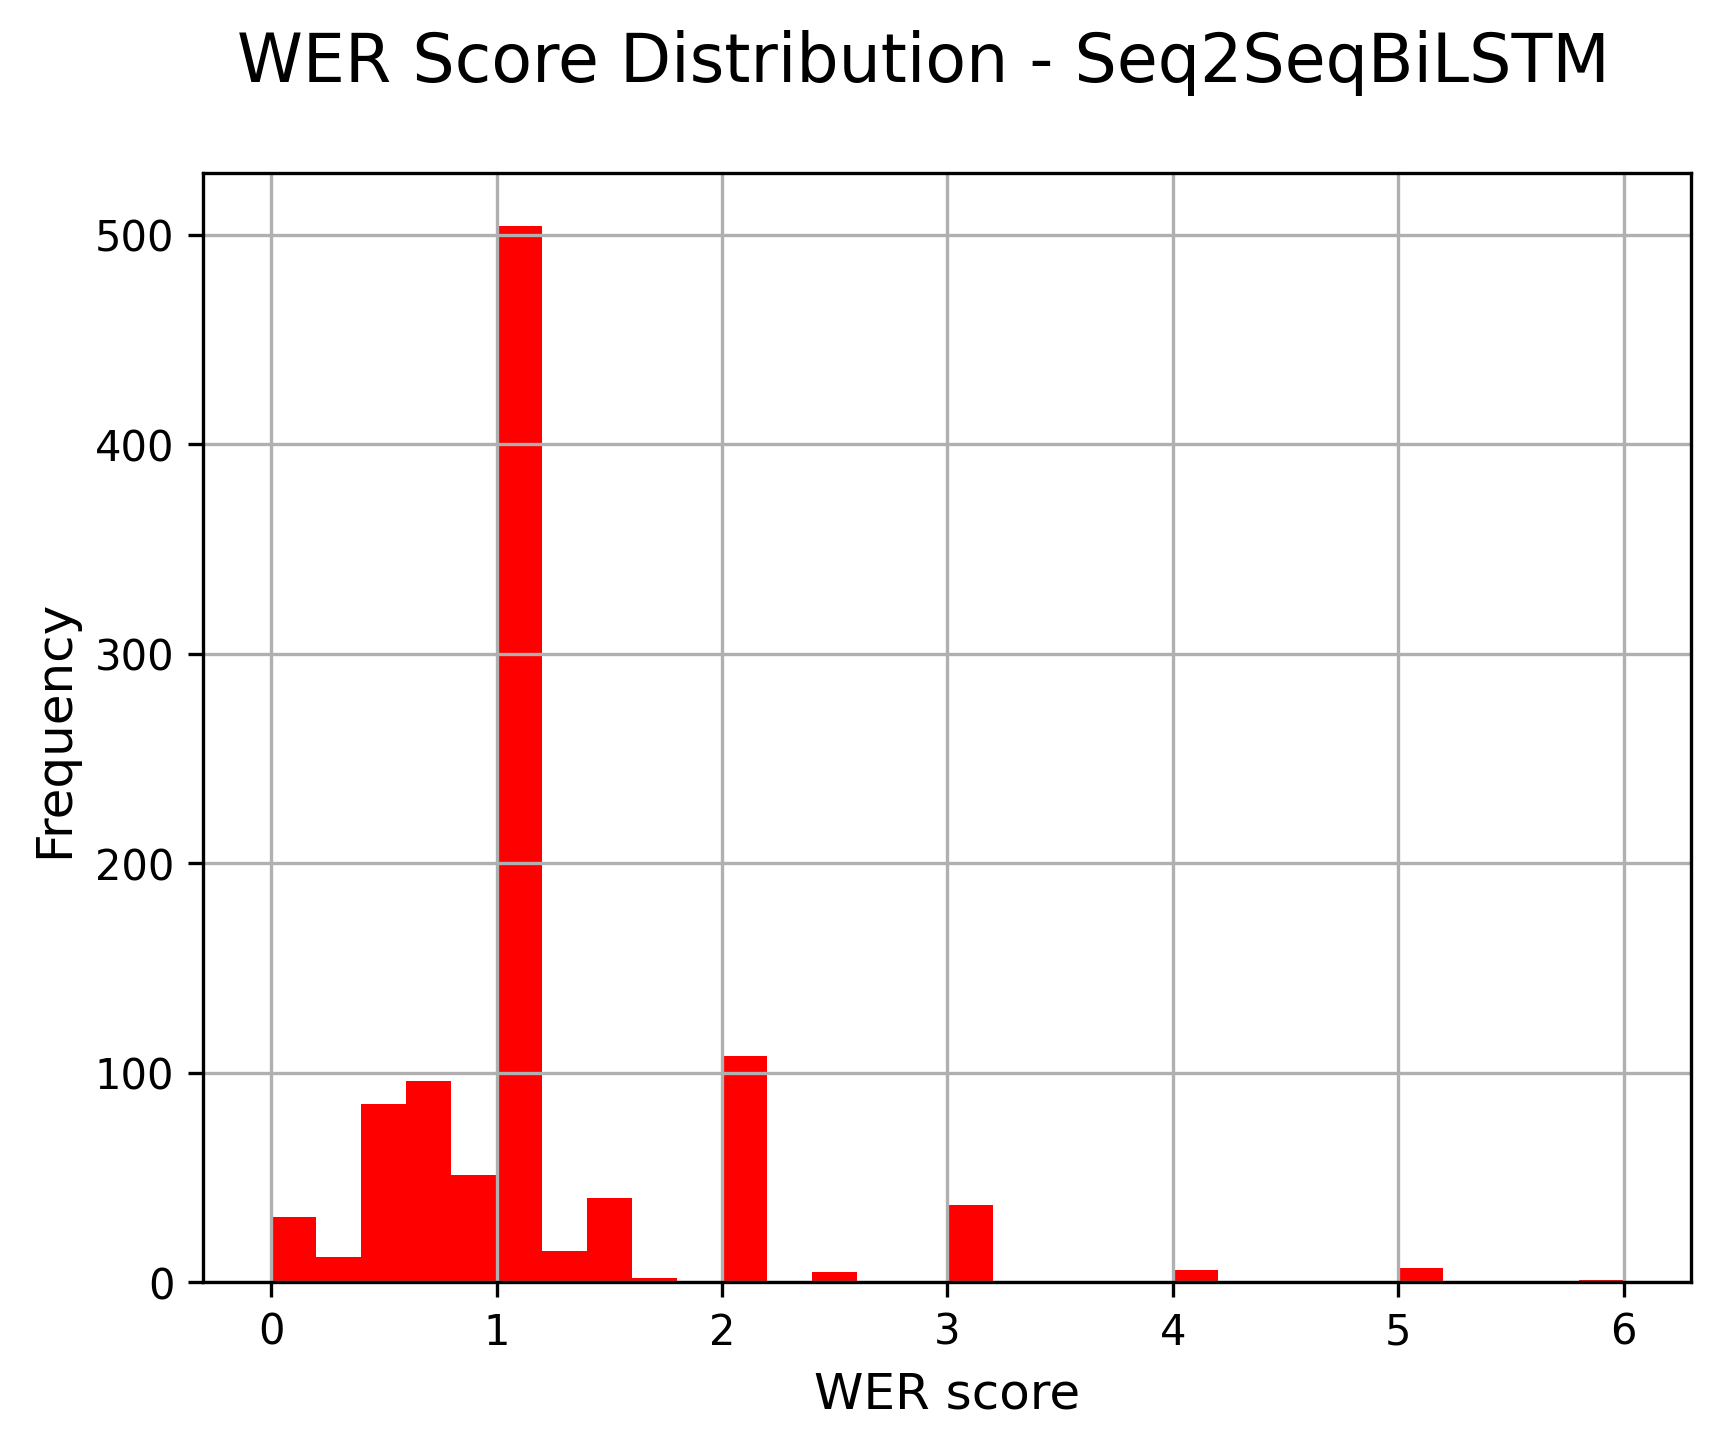
\includegraphics[width=\textwidth]{media/Seq2SeqBiLSTM_wer_scores.png}
        \caption{WER Seq2SeqBiLSTM. Valore medio: 1.1482}
    \end{subfigure}
    \hfill
    \begin{subfigure}{0.22\textwidth}
        \centering
        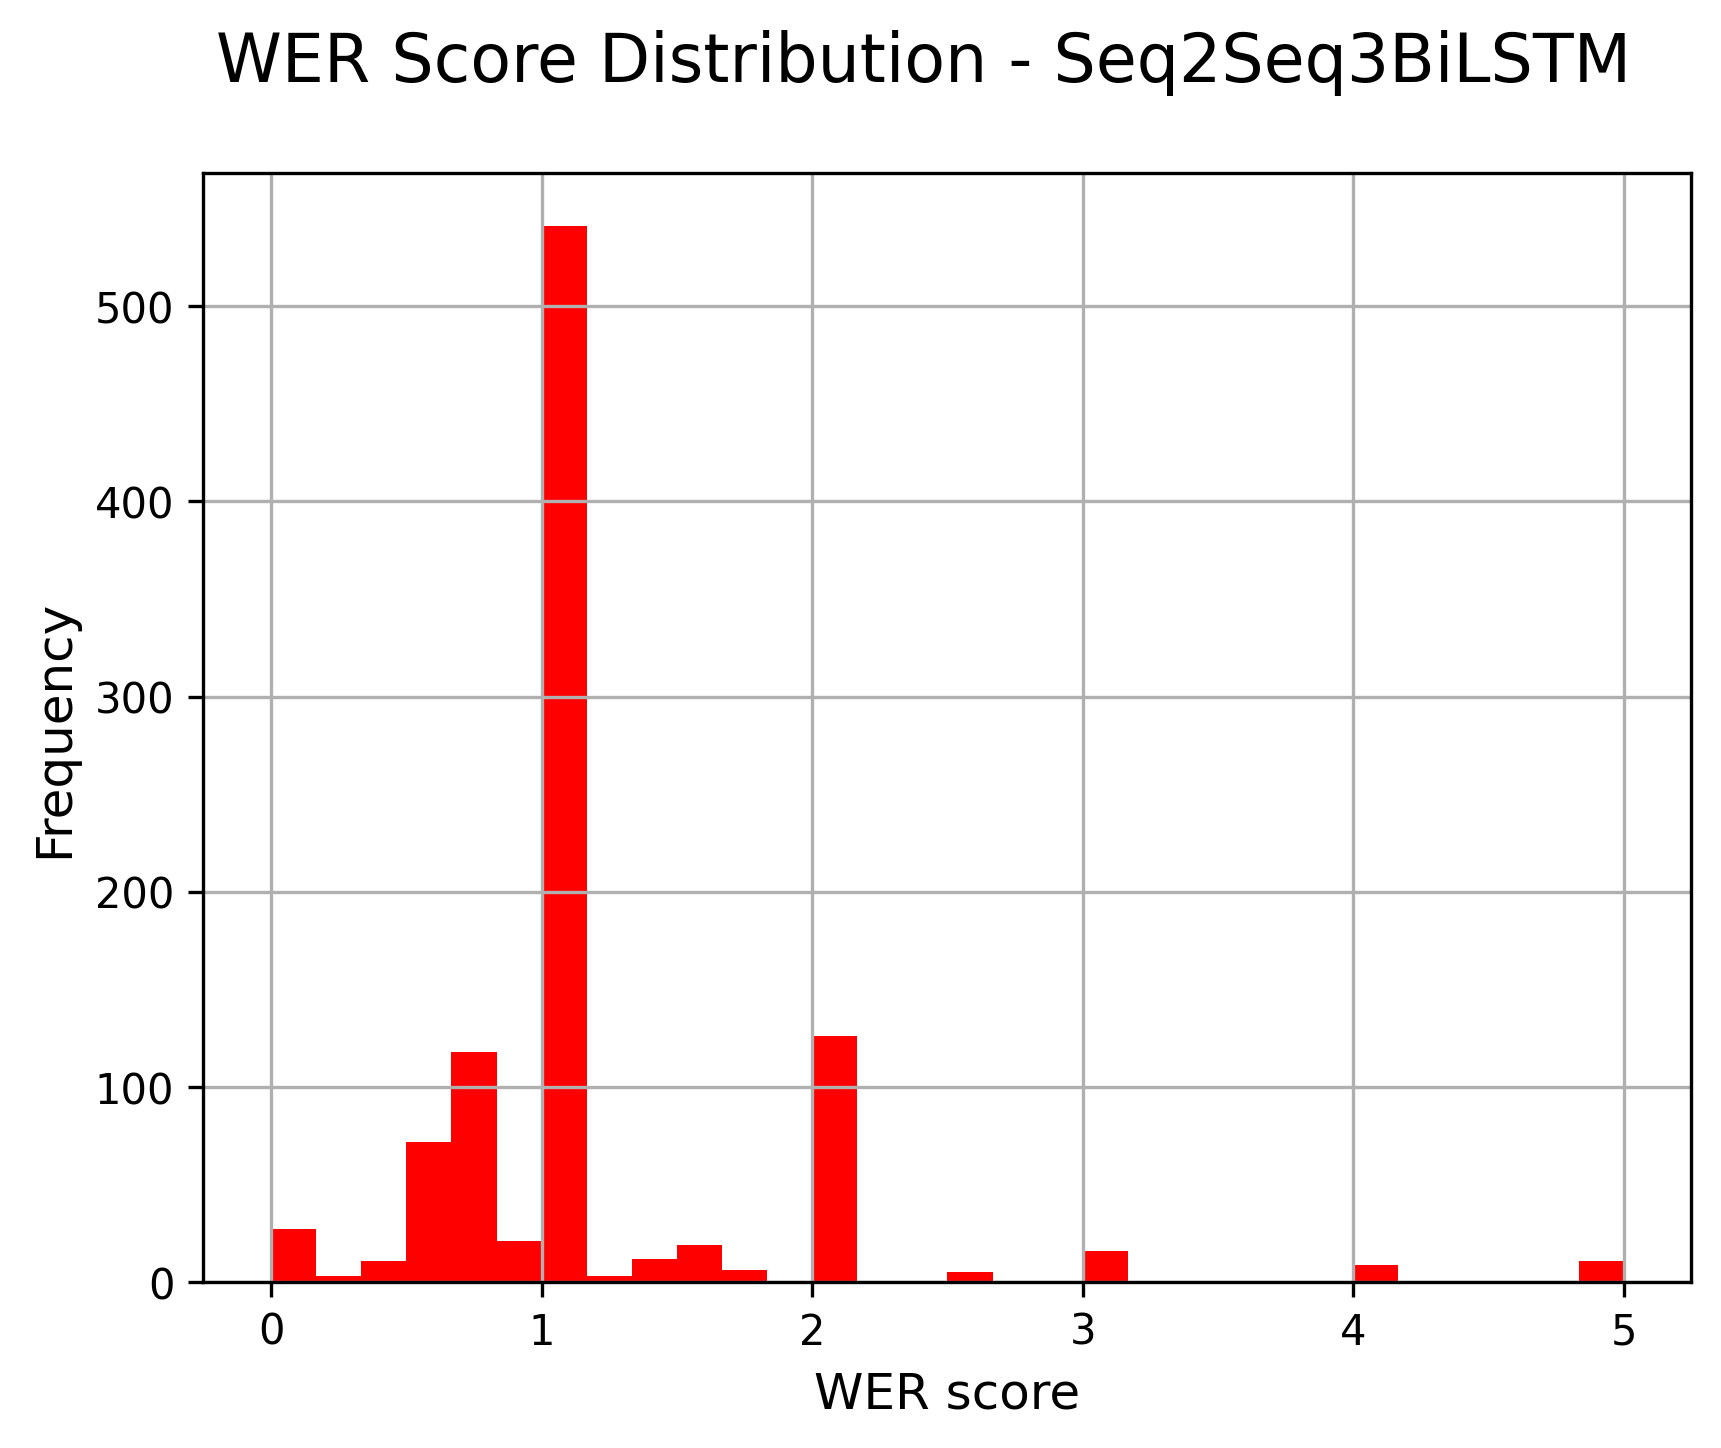
\includegraphics[width=\textwidth]{media/Seq2Seq3BiLSTM_wer_scores.png}
        \caption{WER Seq2Seq3BiLSTM. Valore medio: 1.1474}
    \end{subfigure}
    \hfill
    \begin{subfigure}{0.22\textwidth}
        \centering
        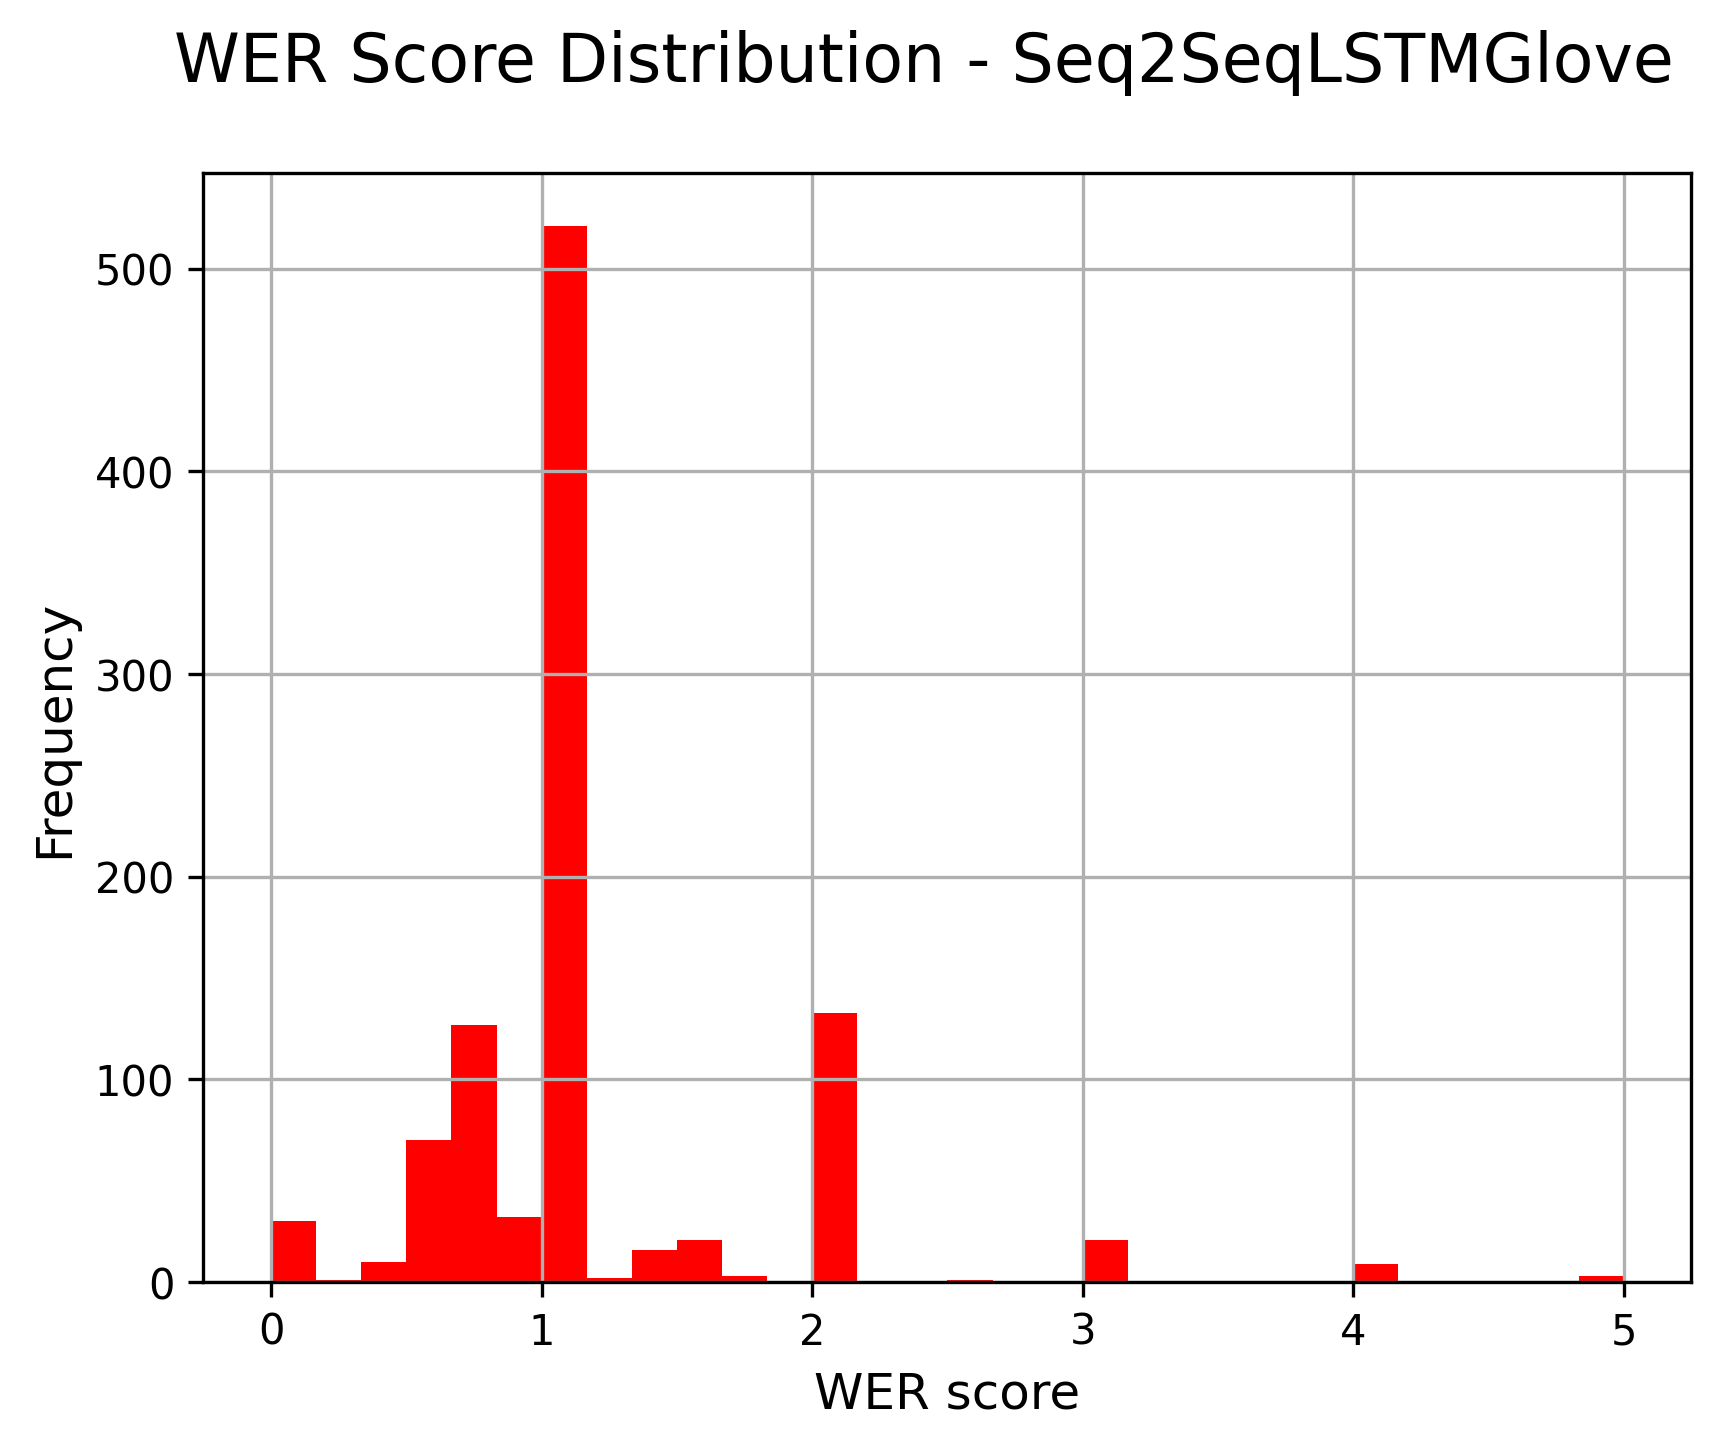
\includegraphics[width=\textwidth]{media/Seq2SeqLSTMGlove_wer_scores.png}
        \caption{WER Seq2SeqLSTMGlove. Valore medio: 1.1456}
    \end{subfigure}
    \hfill
    \begin{subfigure}{0.22\textwidth}
        \centering
        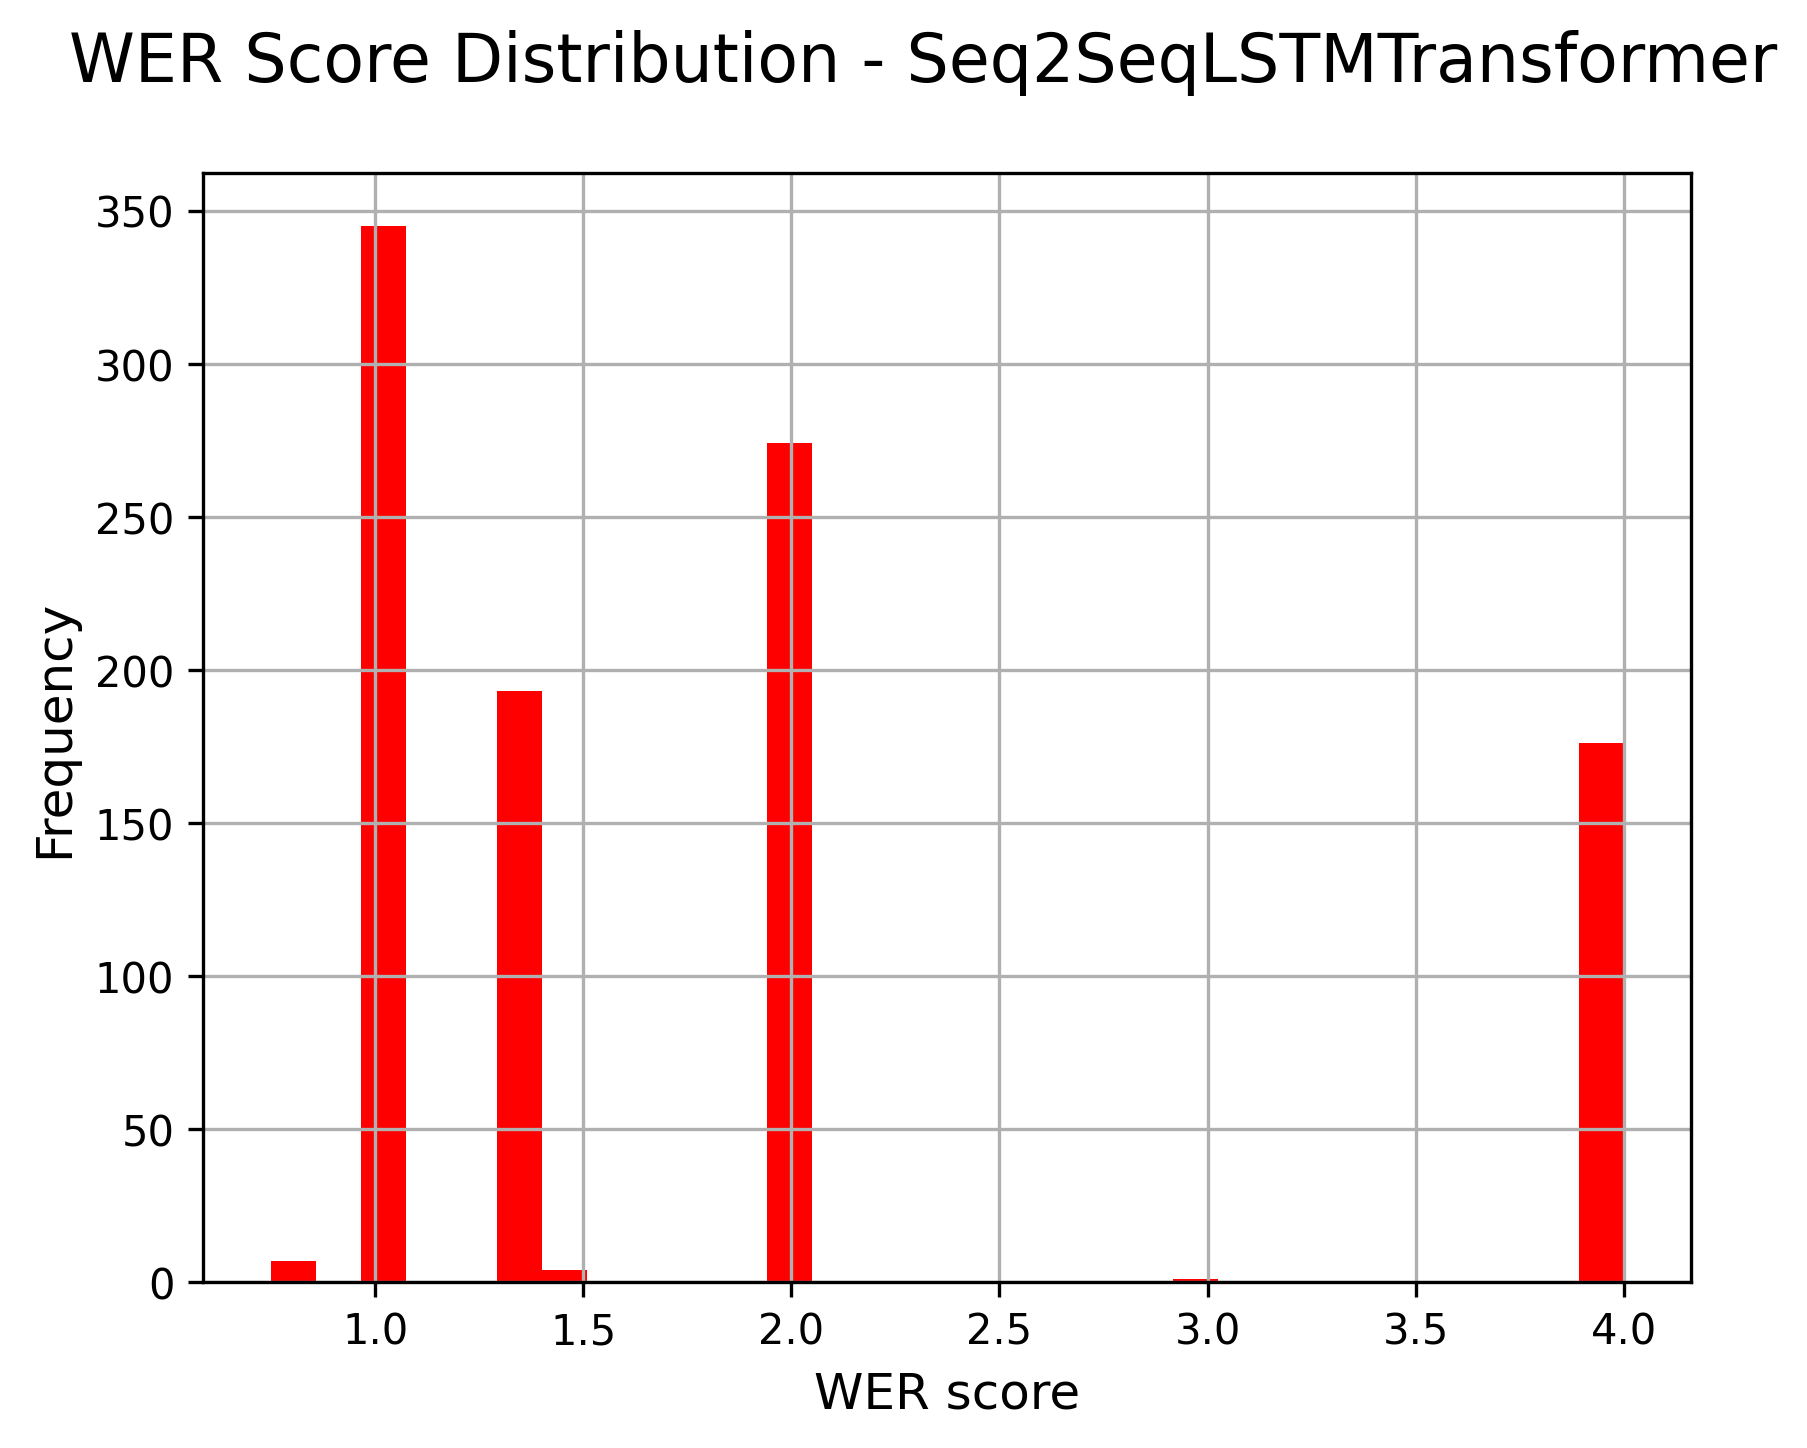
\includegraphics[width=\textwidth]{media/Seq2SeqLSTMTransformer_wer_scores.png}
        \caption{WER Seq2SeqLSTMTransformer. Valore medio: 1.1302}
    \end{subfigure}

    \caption{Confronto del Word Error Rate tra i modelli Seq2SeqLSTM, Seq2SeqBiLSTM, Seq2Seq3BiLSTM, Seq2SeqLSTMGlove e Seq2SeqLSTMTransformer.}
    \label{fig:wer_comparison}
\end{figure}


\subsection{Cosine Similarity}
La similarit\`a cosenica \`e una metrica che calcola la similarit\`a tra due vettori in uno spazio multidimensionale.\\
Nel caso specifico della generazione di riassunti, la similarit\`a cosenica \`e stata calcolata tra i vettori di embedding delle parole nei riassunti generati e quelli nei riassunti di riferimento, con il fine di valutare la qualit\`a dei riassunti generati.\\
La Figura \ref{fig:cosine_similarity_comparison} confronta i valori di similarit\`a cosenica. Anche in questo caso, il modello Seq2SeqBiLSTM ottiene valori pi\`u alti, suggerendo una maggiore correlazione semantica con i riassunti di riferimento.

\begin{figure}[H]
    \centering
    \begin{subfigure}{0.22\textwidth}
        \centering
        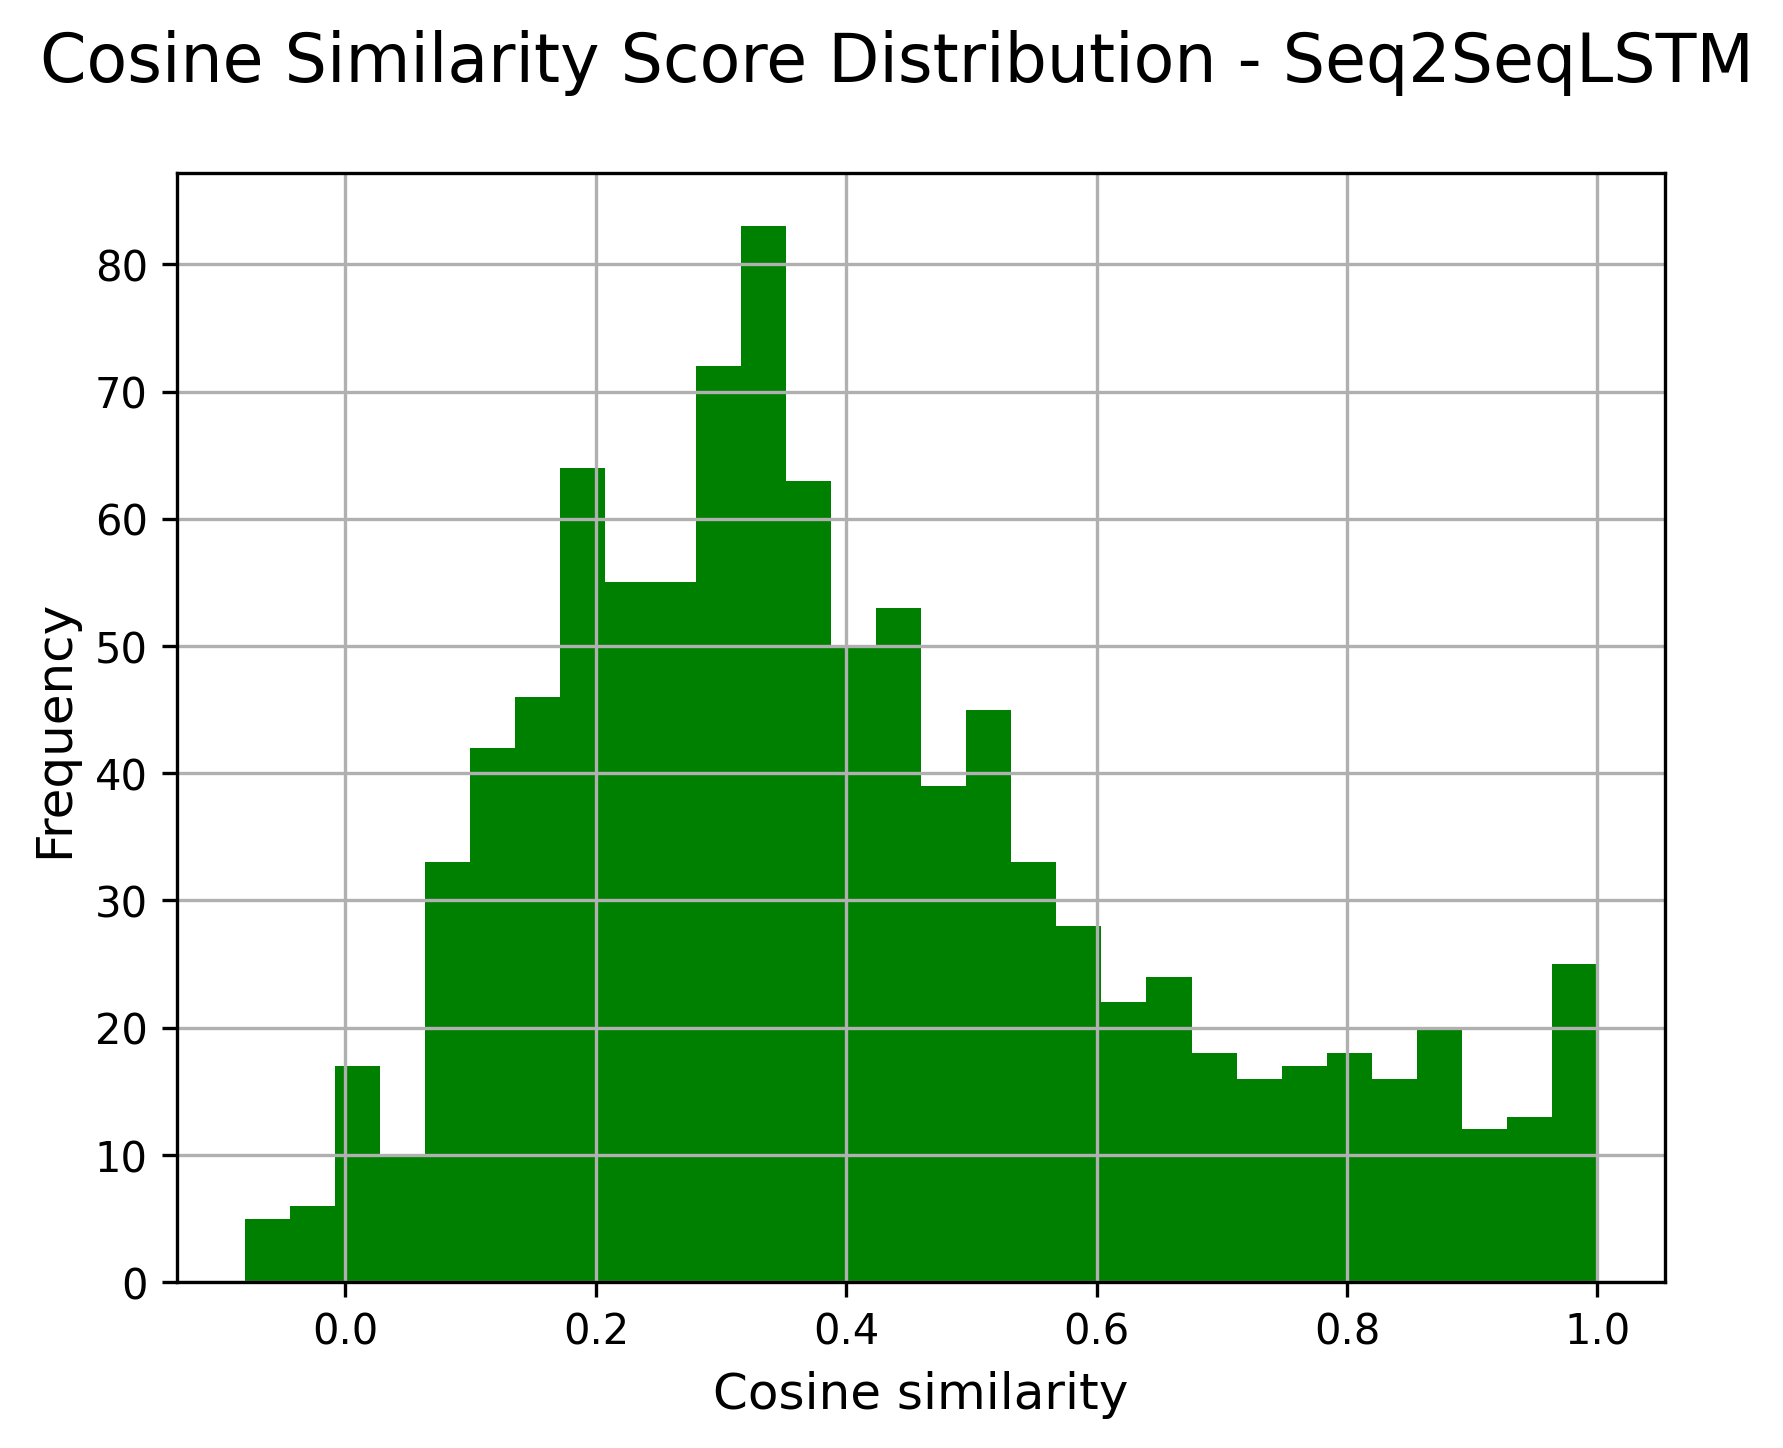
\includegraphics[width=\textwidth]{media/Seq2SeqLSTM_cosine_similarity_scores.png}
        \caption{Cosine Similarity Seq2SeqLSTM. Valore medio: 0.4062}
    \end{subfigure}
    \hfill
    \begin{subfigure}{0.22\textwidth}
        \centering
        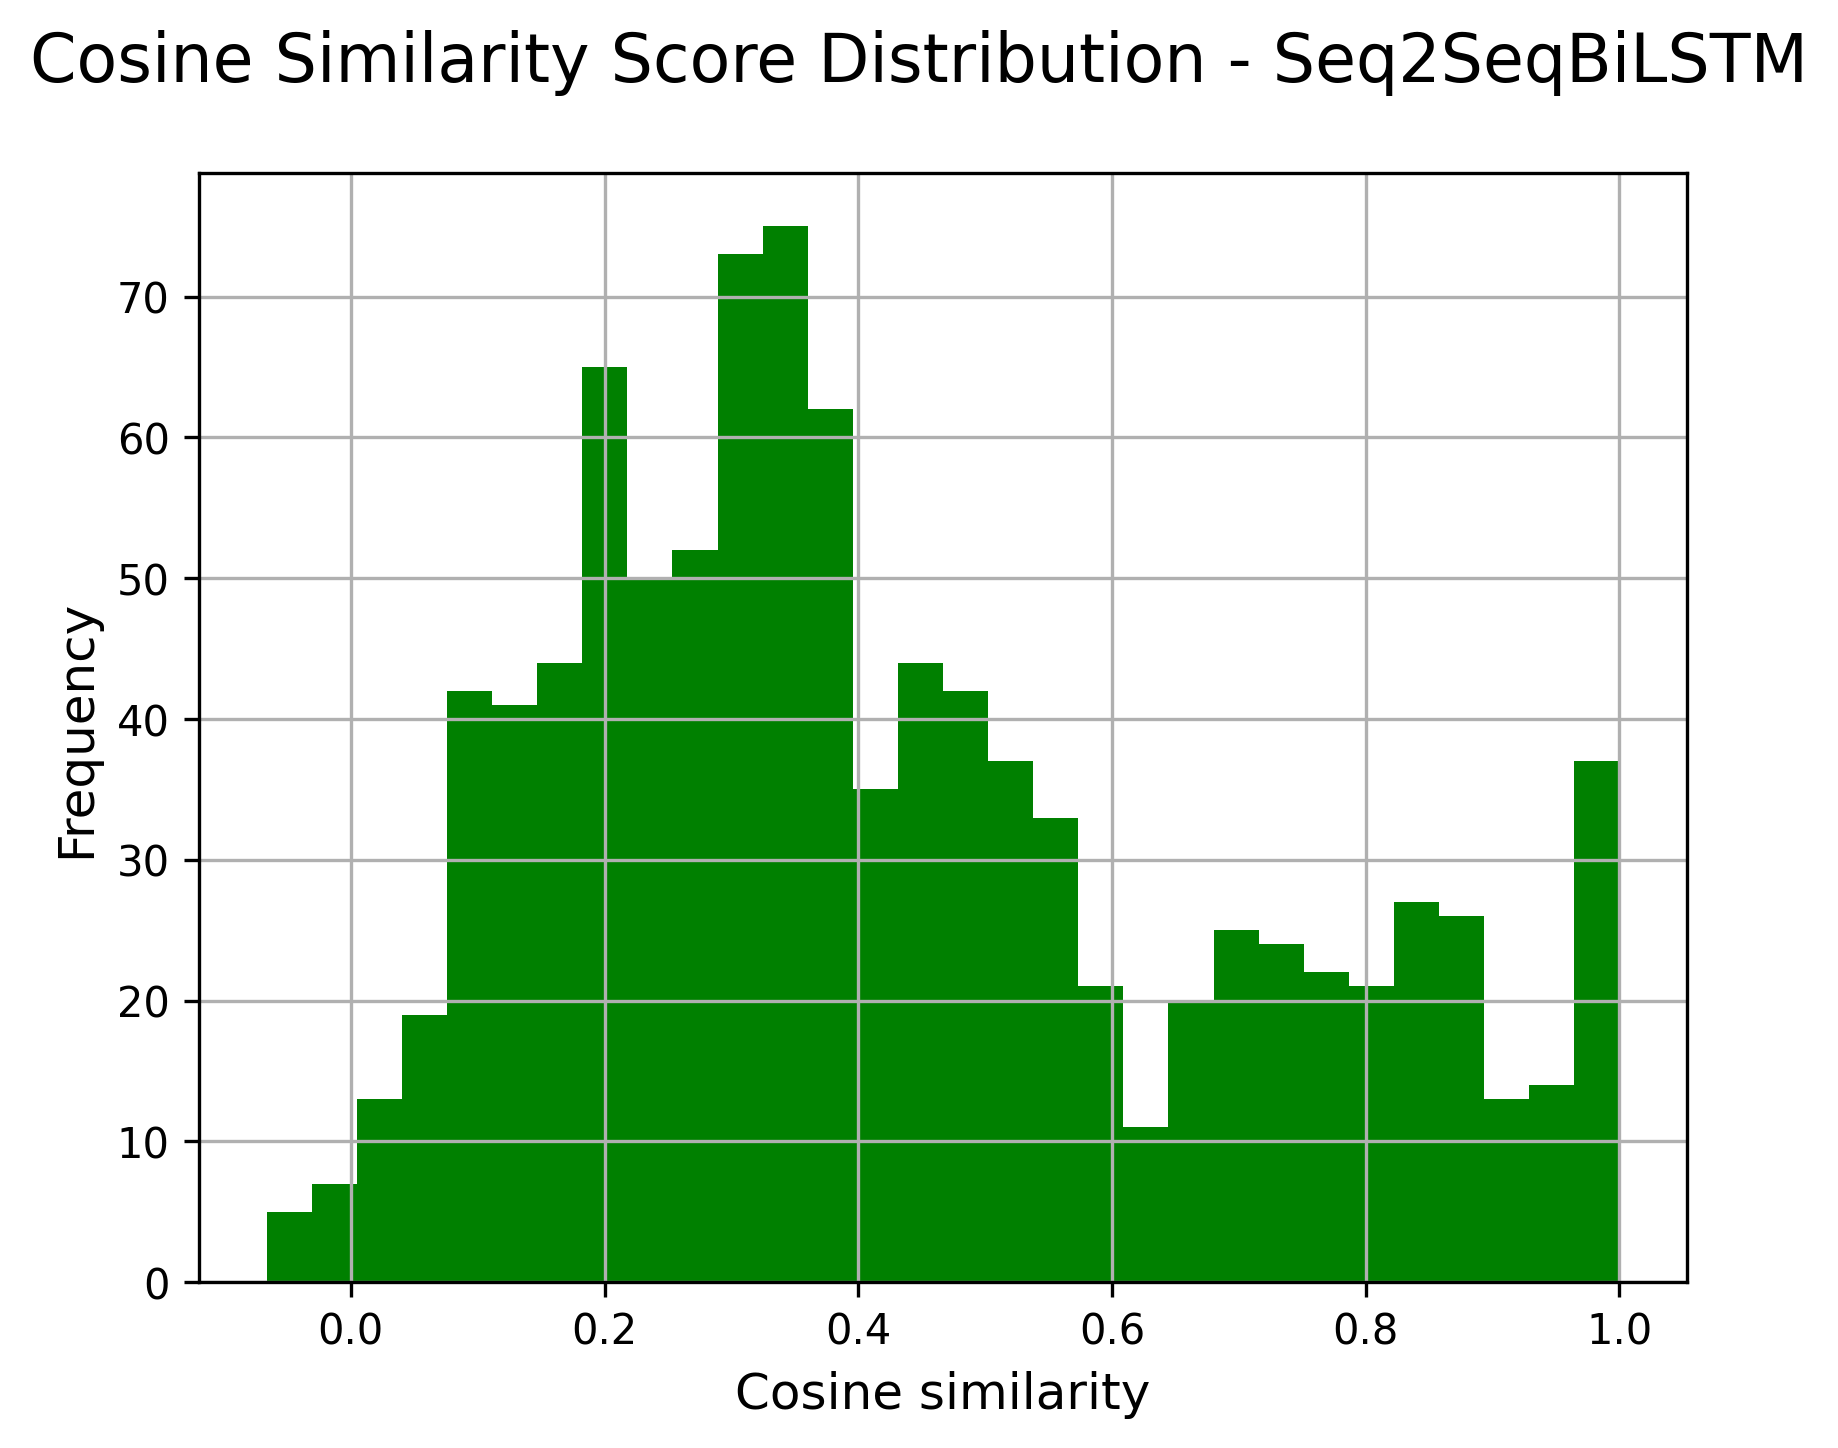
\includegraphics[width=\textwidth]{media/Seq2SeqBiLSTM_cosine_similarity_scores.png}
        \caption{Cosine Similarity Seq2SeqBiLSTM. Valore medio: 0.4289}
    \end{subfigure}
    \hfill
    \begin{subfigure}{0.22\textwidth}
        \centering
        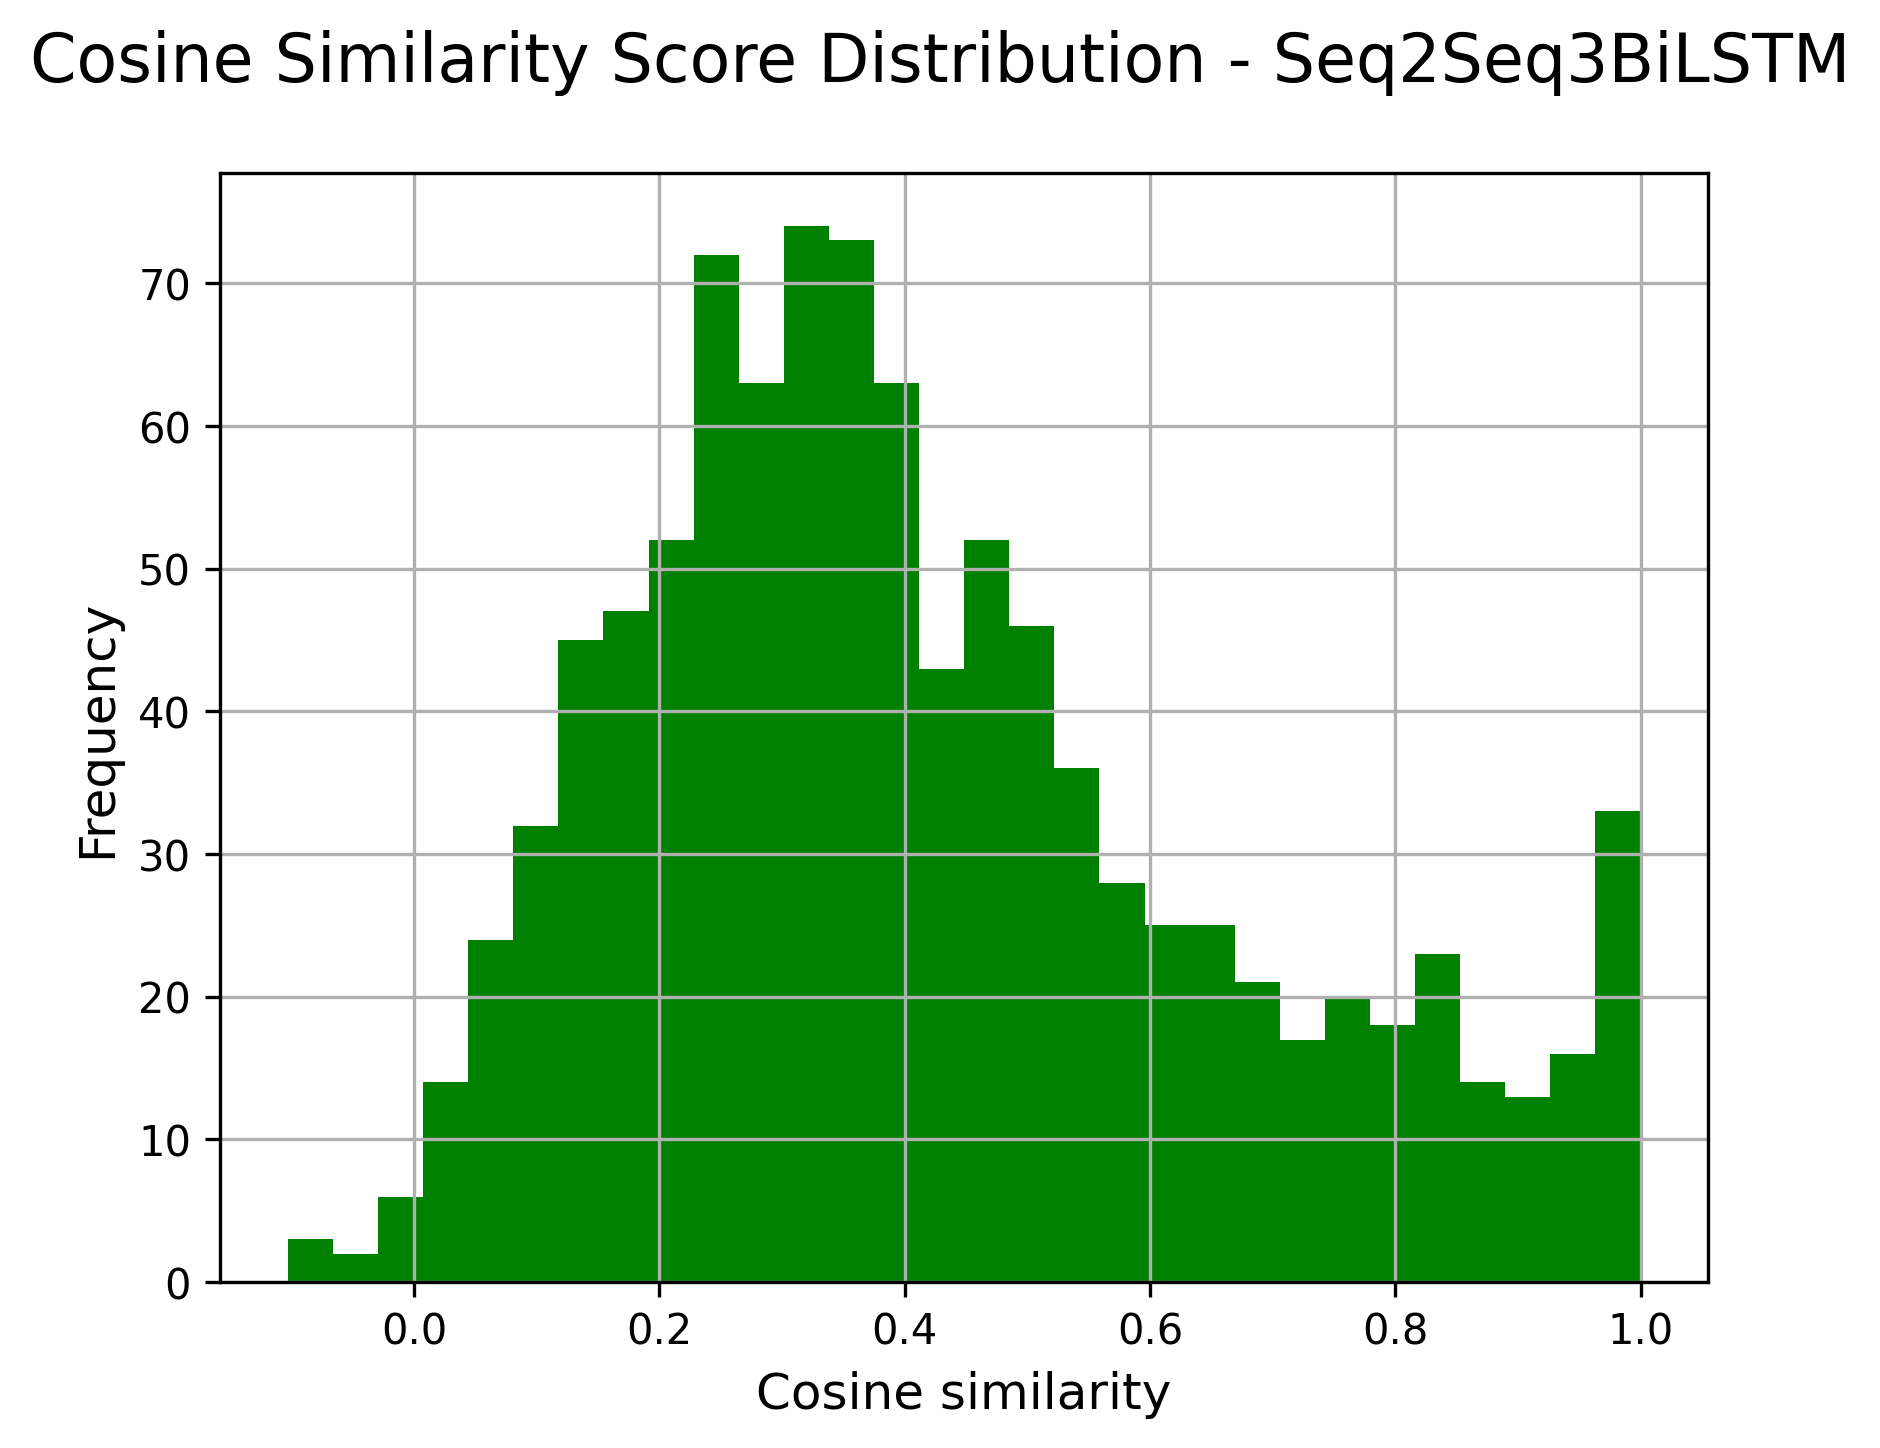
\includegraphics[width=\textwidth]{media/Seq2Seq3BiLSTM_cosine_similarity_scores.png}
        \caption{Cosine Similarity Seq2Seq3BiLSTM. Valore medio: 0.4025}
    \end{subfigure}
    \hfill
    \begin{subfigure}{0.22\textwidth}
        \centering
        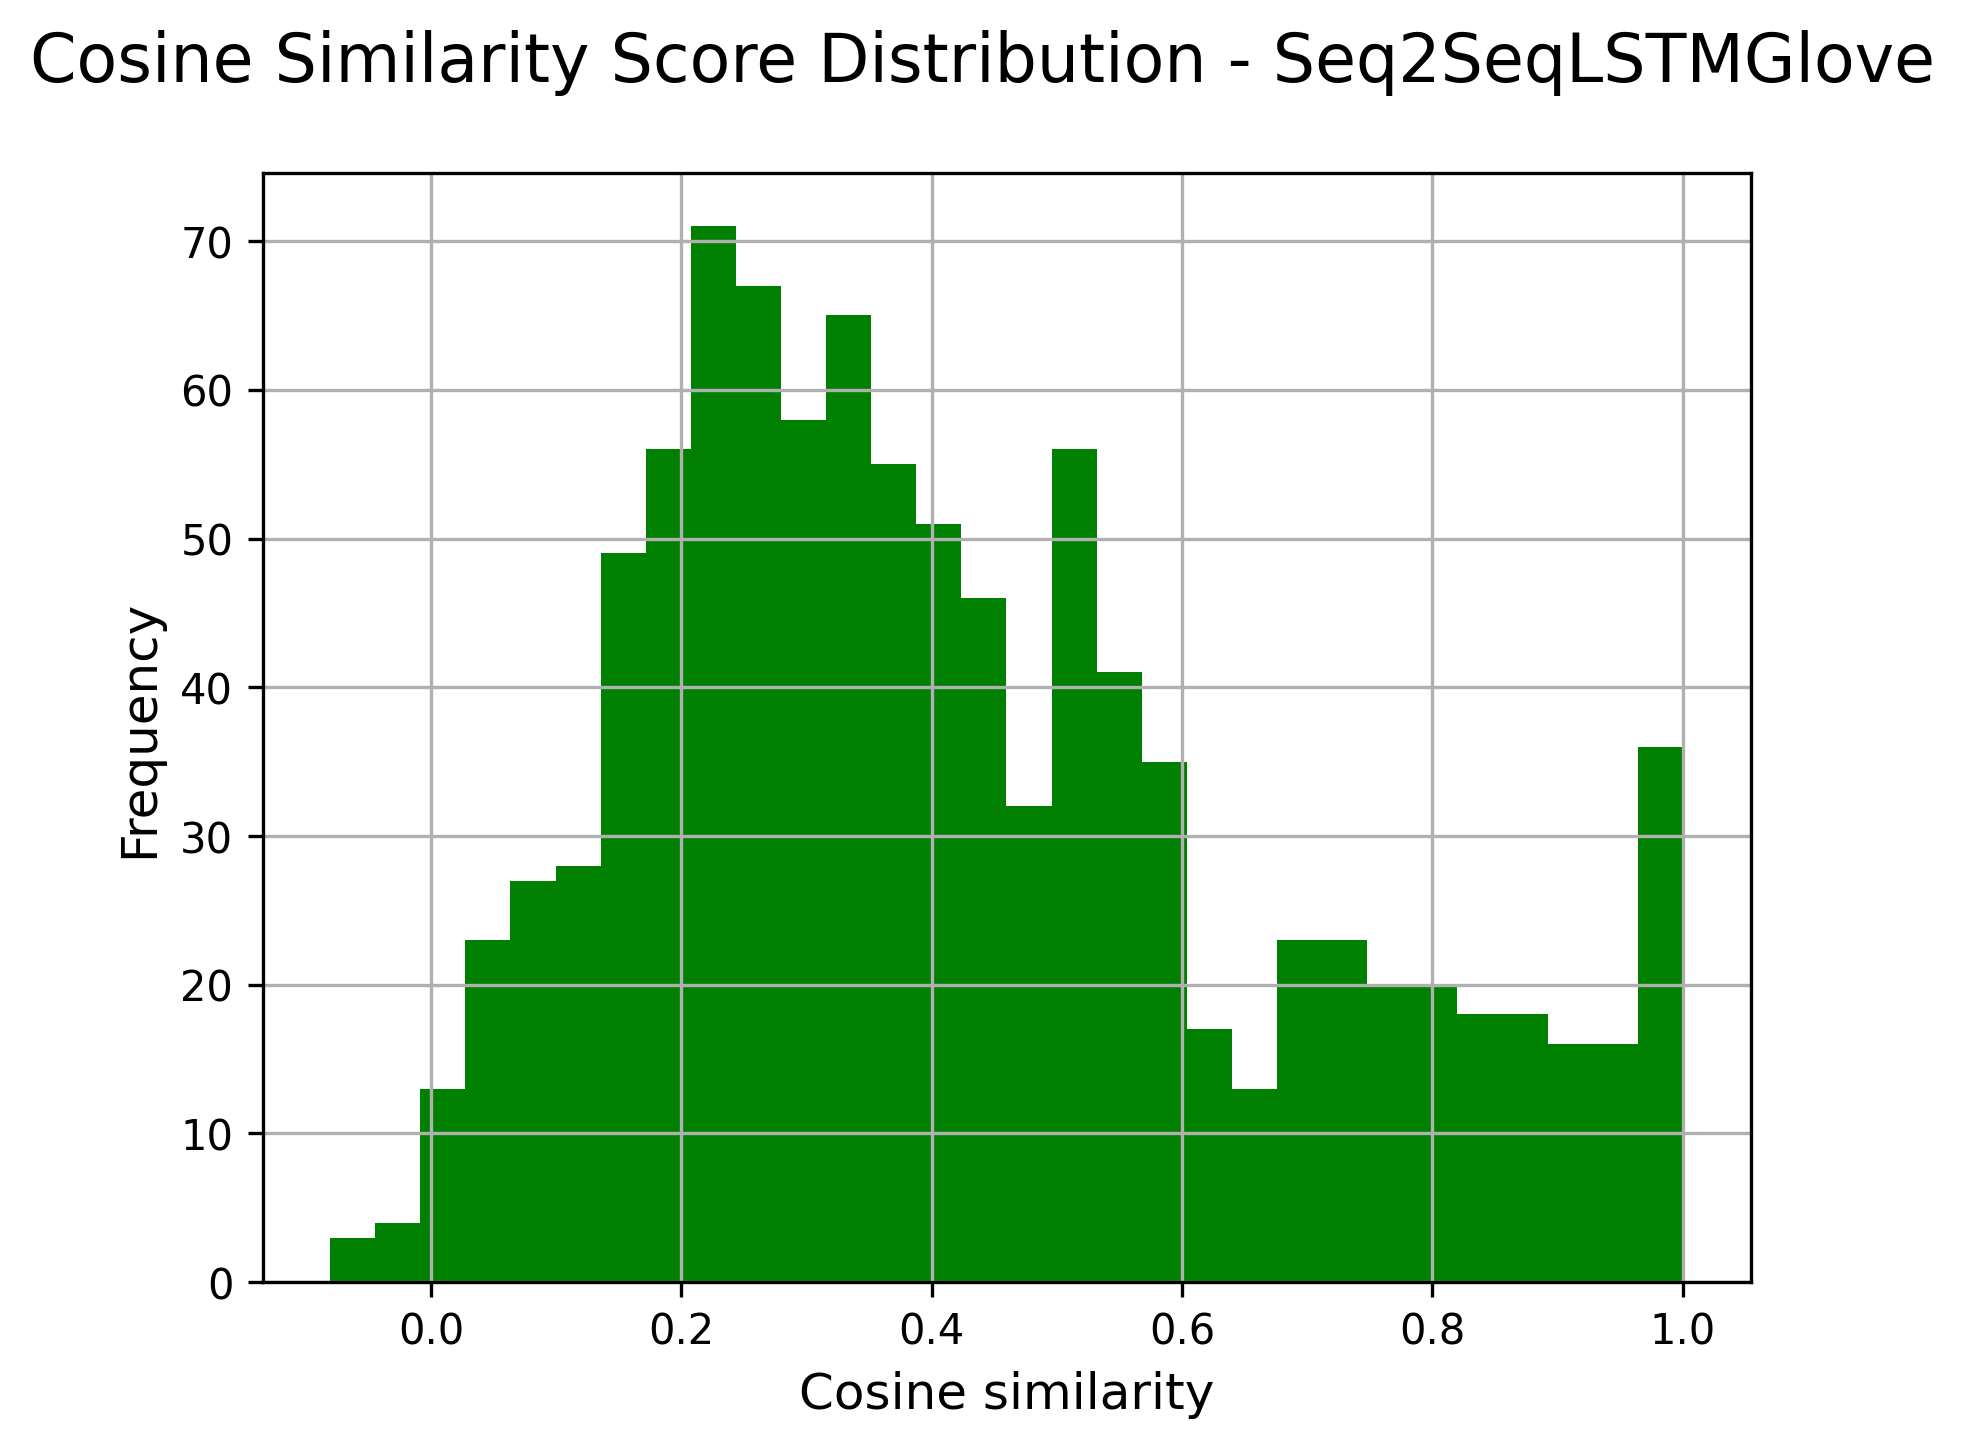
\includegraphics[width=\textwidth]{media/Seq2SeqLSTMGlove_cosine_similarity_scores.png}
        \caption{Cosine Similarity Seq2SeqLSTMGlove. Valore medio: 0.4158}
    \end{subfigure}
    \hfill
    \begin{subfigure}{0.22\textwidth}
        \centering
        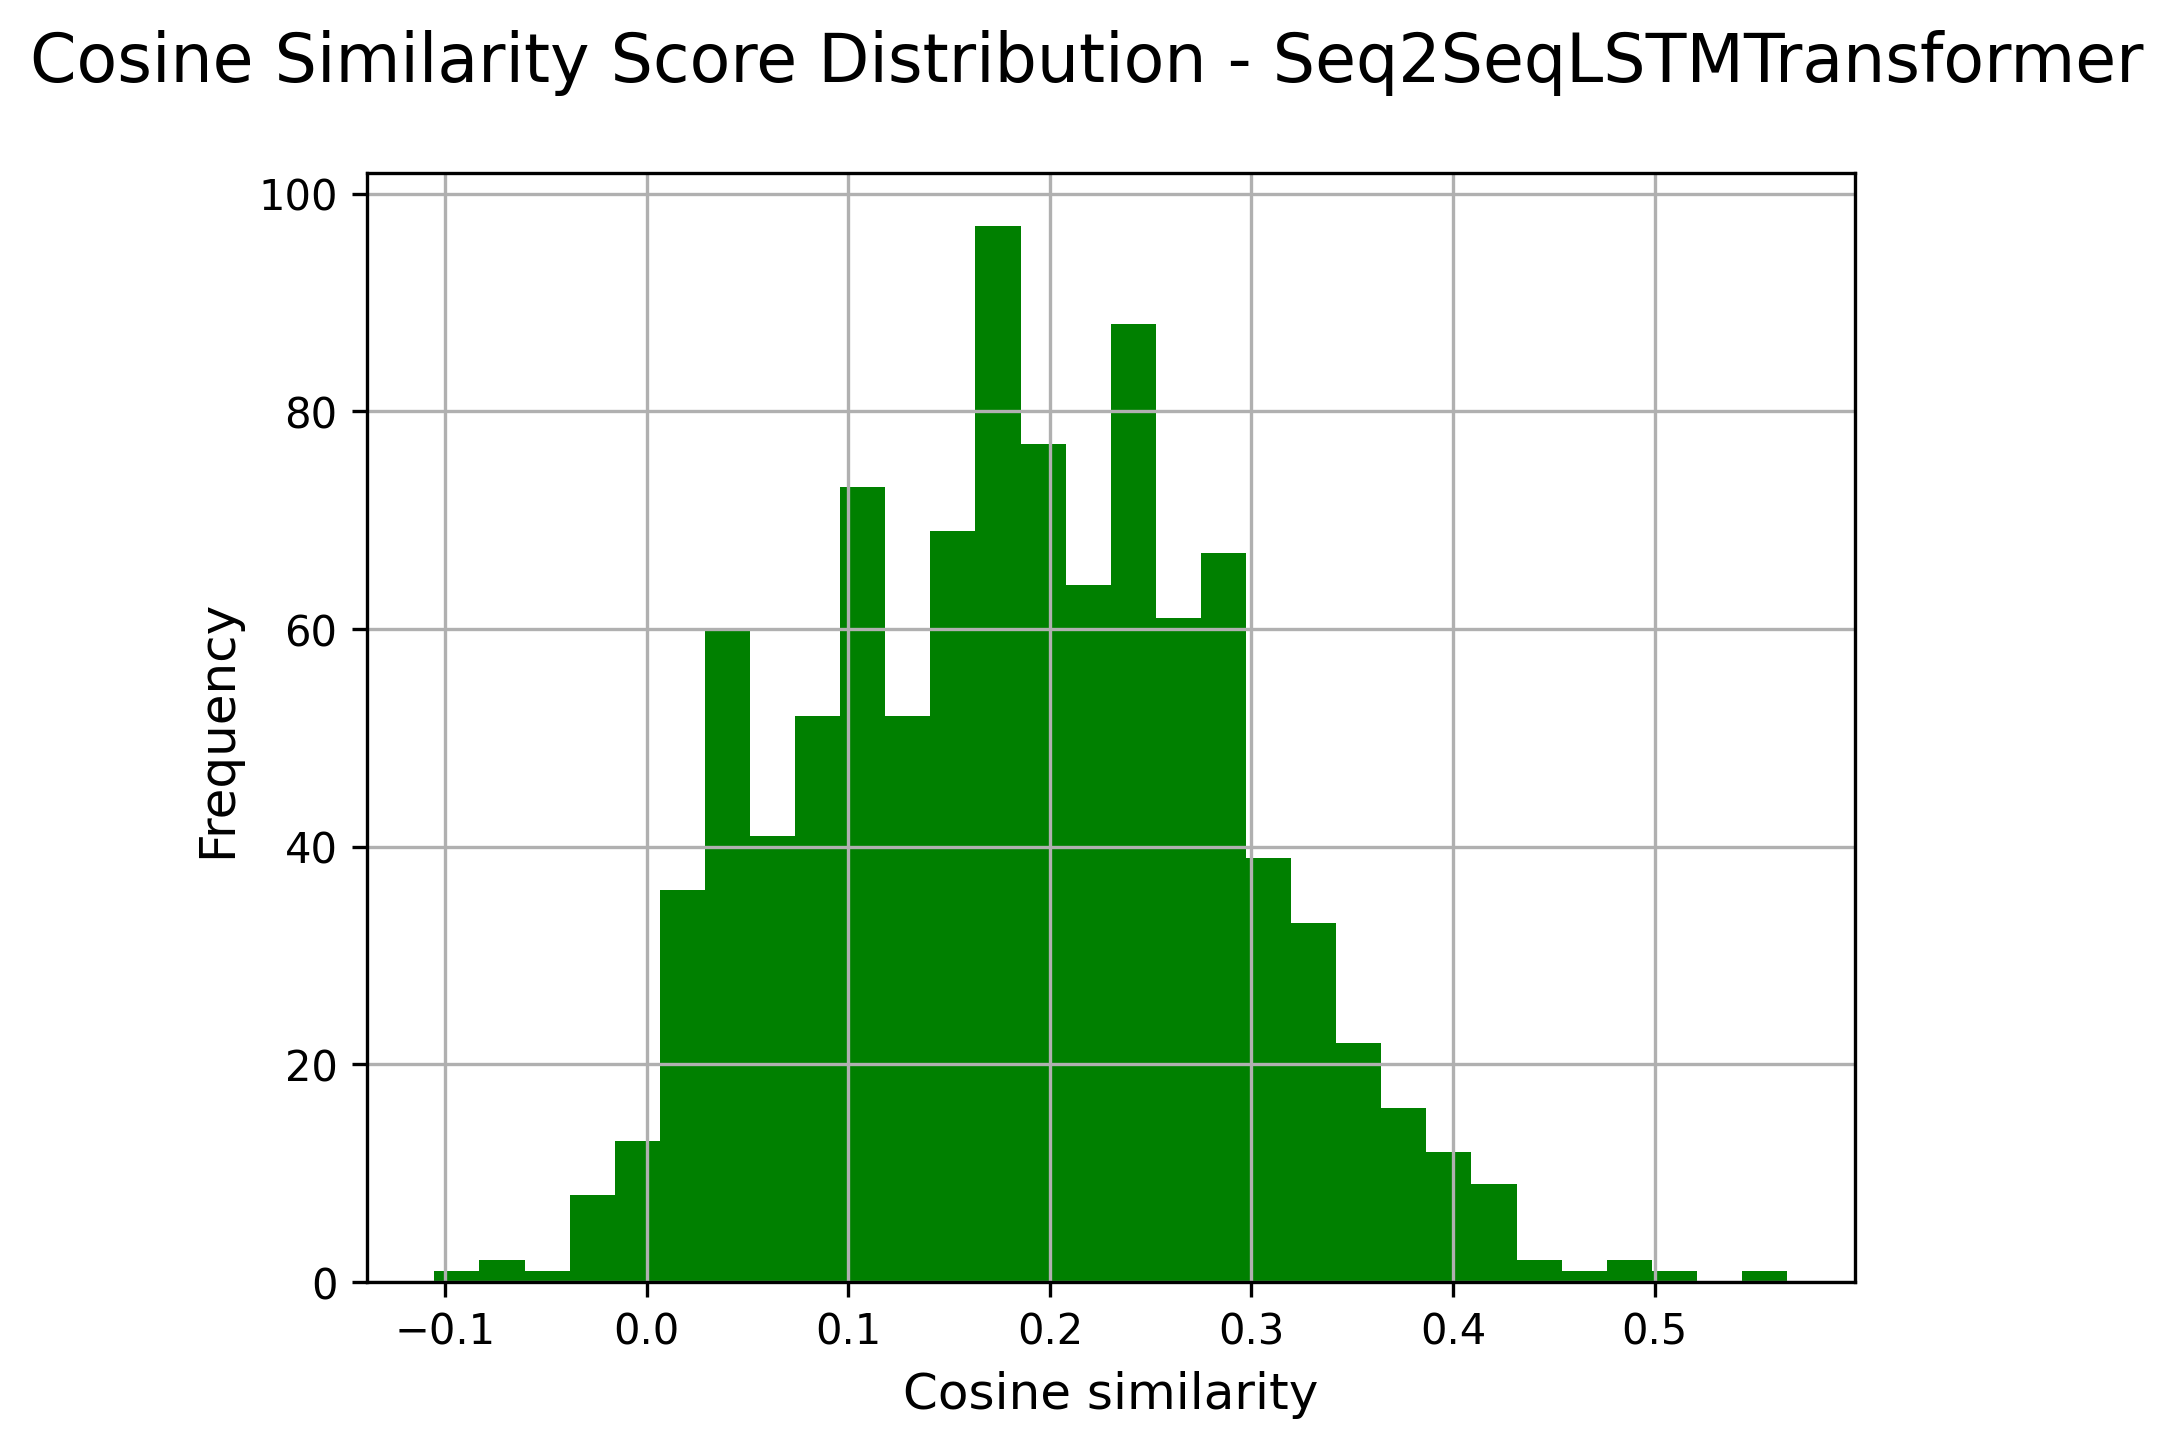
\includegraphics[width=\textwidth]{media/Seq2SeqLSTMTransformer_cosine_similarity_scores.png}
        \caption{Cosine Similarity Seq2SeqLSTMTransformer. Valore medio: 0.4191}
    \end{subfigure}

    \caption{Confronto della cosine similarity tra i modelli Seq2SeqLSTM, Seq2SeqBiLSTM, Seq2Seq3BiLSTM, Seq2SeqLSTMGlove e Seq2SeqLSTMTransformer.}
    \label{fig:cosine_similarity_comparison}
\end{figure}
